\documentclass{beamer}


%\useoutertheme{infoline}
%\useinnertheme{rectangles}
\usepackage{beamerouterthemesplit}
 \useoutertheme{infolines}
\usetheme{Warsaw}

\usepackage[utf8]{inputenc}        
\usepackage[T1]{fontenc}             
% \usepackage[ngerman]{babel}
\usepackage{dsfont}
\usepackage{times}          

\usepackage{amsmath}
\usepackage{mathtools}
\usepackage{amssymb}

\usepackage{pifont}% http://ctan.org/pkg/pifont
\newcommand{\cmark}{\ding{51}}%
\newcommand{\xmark}{\ding{55}}%

\usepackage{bbm}
\usepackage{stmaryrd}
\usepackage{xspace}

\usepackage{hyperref}

\usepackage{tikz}
\usetikzlibrary{
shapes,
shapes.symbols,
shapes.callouts,
arrows,
matrix,
backgrounds,
positioning,
plotmarks,
calc,
patterns,
matrix,
decorations.pathreplacing,
decorations.pathmorphing,
decorations.text,
decorations.shapes,
decorations.fractals,
decorations.markings,
spy
}
\usepackage[colorinlistoftodos,shadow]{todonotes}
\usepackage{listings}

\usepackage{xcolor}
\usepackage{fancyvrb}

\usepackage{tikz-cd}

\newtheorem{defsatzusw}{}
\newtheorem{defi}[defsatzusw]{Definition}
\newtheorem{prop}[defsatzusw]{Proposition}
\newtheorem{satz}[defsatzusw]{Satz}
\newtheorem{bez}[defsatzusw]{Notation}
\newtheorem{bemerkung}[defsatzusw]{Bemerkung}
\newtheorem{lem}[defsatzusw]{Lemma}
\newtheorem{korollar}[defsatzusw]{Corollary}
\newtheorem{myexample}[defsatzusw]{Example}
\newtheorem{konst}[defsatzusw]{Construction}
\newtheorem{notation}[defsatzusw]{Notation}
\newtheorem{eri}[defsatzusw]{Erinnerung}
\newtheorem{remark}[defsatzusw]{Remark}
\newtheorem{sequent}[defsatzusw]{Sequent}
% \newtheorem{block}[defsatzusw]{\phantom{a}}

% \theoremstyle{nonumberbreak}
\newtheorem{bew}{Beweis}
\newtheorem{beweisskizze}{Beweisskizze}

\beamertemplatenavigationsymbolsempty


\newcommand{\N}{\mathbb{N}}
\newcommand{\A}{\mathbb{A}}
\newcommand{\Z}{\mathbb{Z}}
\newcommand{\Q}{\mathbb{Q}}
\newcommand{\R}{\mathbb{R}}
\newcommand{\C}{\mathbb{C}}
\newcommand{\F}{\mathbb{F}}
% \newcommand{\G}{\mathbb{G}}
\newcommand{\Frob}{\phi_q}
\DeclareMathOperator{\kernel}{ker}
\DeclareMathOperator{\im}{im}
\newcommand{\g}{\mathfrak{g}}
\newcommand{\h}{\mathfrak{h}}
\renewcommand{\i}{\mathfrak{i}}
\newcommand{\gl}{\mathfrak{gl}}
\newcommand{\n}{\mathfrak{n}}
\newcommand{\nminus}{\mathfrak{n}_{-}}
\renewcommand{\sl}{\mathfrak{sl}}
\newcommand{\slz}{\mathfrak{sl}_2}
% \newcommand{\b}{\mathfrak{b}}

\DeclareMathOperator{\domain}{dom}
\DeclareMathOperator{\defect}{def}
\DeclareMathOperator{\GL}{GL}
\DeclareMathOperator{\Det}{det}
\DeclareMathOperator{\Mon}{Mon}
\DeclareMathOperator{\ggt}{ggT}
\DeclareMathOperator{\Min}{min}
\DeclareMathOperator{\conv}{conv}
\DeclareMathOperator{\New}{New}
\DeclareMathOperator{\supp}{supp}
\DeclareMathOperator{\voln}{Vol_n}
\DeclareMathOperator{\volnn}{Vol_{n-1}}
\DeclareMathOperator{\MV}{MV}
\DeclareMathOperator{\Dim}{dim}
\DeclareMathOperator{\SMV}{SMV}
\DeclareMathOperator{\sgn}{Signum}
\DeclareMathOperator{\Null}{Null}
\DeclareMathOperator{\Pot}{Pot}
\DeclareMathOperator{\Ass}{Ass}
\DeclareMathOperator{\Rg}{Rg}
\DeclareMathOperator{\codim}{codim}
\DeclareMathOperator{\vol2}{Vol_{2}}
\DeclareMathOperator{\Char}{Char}
\DeclareMathOperator{\Div}{Div}
\DeclareMathOperator{\CDiv}{CDiv}
\DeclareMathOperator{\Pic}{Pic}
\DeclareMathOperator{\Kern}{Kern}
\DeclareMathOperator{\Kokern}{Kokern}
\DeclareMathOperator{\Bild}{Bild}
\DeclareMathOperator{\Cl}{Cl}
\DeclareMathOperator{\Spec}{Spec}
\DeclareMathOperator{\Kegel}{Kegel}
\DeclareMathOperator{\Hom}{Hom}
\DeclareMathOperator{\Aut}{Aut}
\DeclareMathOperator{\Gal}{Gal}
\DeclareMathOperator{\Quot}{Quot}
\DeclareMathOperator{\Lie}{L}
\DeclareMathOperator{\Stab}{Stab}
\DeclareMathOperator{\chars}{Char}
\DeclareMathOperator{\divis}{div}
\DeclareMathOperator{\Cone}{Cone}
\DeclareMathOperator{\rk}{rk}
\DeclareMathOperator{\Fix}{Fix}
\DeclareMathOperator{\Weyl}{W}
\DeclareMathOperator{\Coxeter}{C}
\DeclareMathOperator{\End}{End}
\DeclareMathOperator{\ad}{ad}
\DeclareMathOperator{\tr}{tr}
\DeclareMathOperator{\coker}{coker}
\DeclareMathOperator{\G}{G}
\DeclareMathOperator{\CH}{H}
\DeclareMathOperator{\id}{id}
\DeclareMathOperator{\Sh}{Sh}
\DeclareMathOperator{\grmod}{grmod}
\DeclareMathOperator{\Projectives}{Projectives}
\DeclareMathOperator{\Tot}{Tot}
\DeclareMathOperator{\Image}{im}
\DeclareMathOperator{\Kernel}{ker}
\DeclareMathOperator{\KernelEmbedding}{KernelEmbedding}
\DeclareMathOperator{\KernelObject}{KernelObject}
\DeclareMathOperator{\KernelLift}{KernelLift}

\renewcommand{\P}{\mathbb{P}}
\renewcommand{\phi}{\varphi}

\newcommand{\mathO}[1]{\mathcal{O}_{#1}}
\xdefinecolor{darkgreen}{RGB}{175, 193, 36}
\definecolor{forestgreen}{RGB}{173,255,47}
\newcommand{\myblue}{blue!15}

\newcommand{\CategoriesForHomalg}{\texttt{Categories} }
\newcommand{\CapPkg}{\textsc{Cap}\xspace}
\newcommand{\Gap}{\textsc{Gap}\xspace}
\newcommand{\ToolsForHomalg}{\texttt{ToolsForHomalg} }

\definecolor{objects}{cmyk}{.25,1,.7,.2}
\definecolor{morphisms}{cmyk}{1,.4,1,0}
\definecolor{later_morphisms}{cmyk}{.6,0,1,0}
\definecolor{later_arrow}{cmyk}{0,.59,1,.12}
\definecolor{darkgray}{rgb}{0.3,0.3,0.3}

\definecolor{computerfriendly}{cmyk}{.6,0,1,0}
\definecolor{computerfriendlymor}{rgb}{0.3,0.3,1}

\newcommand{\FiberProduct}{\mathrm{FiberProduct}}
\newcommand\Rpres{{\ensuremath{R\mathrm{\textnormal{-}fpres}}}\xspace}
\newcommand{\Obj}{\mathrm{Obj}}
\newcommand{\Mor}{\mathrm{Mor}}
\newcommand{\Int}{\mathrm{Int}}
\newcommand{\ListObj}{\mathrm{ListObj}}
\newcommand{\Pushout}{\mathrm{Pushout}}
\newcommand{\KernelEmb}{\mathrm{KernelEmb}}
\newcommand{\DirectProduct}{\mathrm{DirectProduct}}
\newcommand{\TerminalObject}{\mathrm{TerminalObject}}
\newcommand{\PreCompose}{\mathrm{PreCompose}}
\newcommand{\ProjectionInFactor}{\mathrm{ProjectionInFactor}}
\newcommand{\Efpgrmod}{\wedge V\textnormal{-}\mathrm{grmod}}
\newcommand{\EGfpgrmod}{\wedge V\rtimes G\textnormal{-}\mathrm{grmod}}
\newcommand{\Coh}{\mathfrak{Coh}}
\newcommand{\Pro}{\mathbb{P}}
\newcommand{\Gen}[1]{\G ( \mathcal{#1} ) }

% \newcommand{\SeppVisible}[2]{\visible<\textsl{\detokenize{#1}}>{#2}}
\newcommand{\visiblethree}[1]{\visible<3->{#1}}
\newcommand{\visiblefour}[1]{\visible<4->{#1}}
\newcommand{\visiblefive}[1]{\visible<5->{#1}}
\newcommand{\visiblesix}[1]{\visible<6->{#1}}
\newcommand{\visibleseven}[1]{\visible<7->{#1}}
\newcommand{\visibleeight}[1]{\visible<8->{#1}}
\newcommand{\visiblenine}[1]{\visible<9->{#1}}
\newcommand{\visibleten}[1]{\visible<10->{#1}}
\newcommand{\visibleeleven}[1]{\visible<11->{#1}}
\newcommand{\visiblethirteen}[1]{\visible<13->{#1}}
\newcommand{\visiblefifteen}[1]{\visible<15->{#1}}

\newcommand{\intExt}{\mathcal{E}xt}
\newcommand{\intHom}{\mathcal{H}om}

\newcommand*{\ifactor}{1.5}%
\newcommand{\dashdownarrow}{\raisebox{2.0ex}{\rotatebox{-90}{$\dashrightarrow$}}}
\newcommand{\stgrmod}{\text{-}\underline{\smash{\mathrm{grmod}}}}
\newcommand{\SRep}{\mathrm{{{\color{computerfriendly}S}}Rep}_{k}}

\newcommand{\kxnpgrmod}{{{\ensuremath{K\left[x_1,\dots,x_{n+1}\right]\mathrm{\textnormal{-}grmod}}}\xspace}}
\newcommand{\kxngrmod}{{{\ensuremath{K\left[x_1,\dots,x_{n}\right]\mathrm{\textnormal{-}grmod}}}\xspace}}
\newcommand{\kxnmod}{{{\ensuremath{K\left[x_1,\dots,x_{n}\right]\mathrm{\textnormal{-}mod}}}\xspace}}
\newcommand{\sgrmod}{{{\ensuremath{S\mathrm{\textnormal{-}grmod}}}\xspace}}
\newcommand{\sgrmodred}{{{\ensuremath{S\mathrm{\textnormal{-}{\color{red}grmod}}}}\xspace}}
\newcommand{\smod}{{{\ensuremath{S\mathrm{\textnormal{-}mod}}}\xspace}}

\newcommand{\kvec}{k\mathrm{\text{-}vec}}
\DeclareMathOperator{\Irr}{\mathrm{Irr}}
\newcommand{\Rep}{\mathrm{Rep}_{k}}
\renewcommand{\P}{\mathbb{P}}
\renewcommand{\phi}{\varphi}

\newcommand{\modZ}{\mathrm{mod}_{\Z}}
\newcommand{\modR}{\mathrm{mod}_{R}}
\newcommand{\pmatrow}[2]{ \begin{pmatrix}{#1} & {#2} \end{pmatrix} }
\newcommand{\pmatcol}[3]{ \scriptsize\begin{pmatrix}{#1} \\ {#2} \\ {#3}\end{pmatrix} }
\newcommand{\fpresR}{\mathrm{fpres}_{R}}
  
\defbeamertemplate{section page}{mine}[1][]{%
  \begin{centering}
    {\usebeamerfont{section name}\usebeamercolor[fg]{section name}#1}
    \vskip1em\par
    \begin{beamercolorbox}[sep=12pt,center]{part title}
      \usebeamerfont{section title}\insertsection\par
    \end{beamercolorbox}
  \end{centering}
}

\setbeamertemplate{section page}[mine]

\AtBeginPart{\frame{\partpage}}
\AtBeginSection{
\begin{frame}
 \frametitle{}
 \tableofcontents[currentsection]
\end{frame}
}
\AtBeginSubsection{
\begin{frame}
 \frametitle{}
 \tableofcontents[currentsection,currentsubsection]
\end{frame}
}

\title[Constructive categories]{Constructive category theory with \CapPkg}
\author[Gutsche, Posur]{Sebastian Gutsche and Sebastian Posur}
\date[May 10, 2019]{May 10, 2019}
\titlegraphic{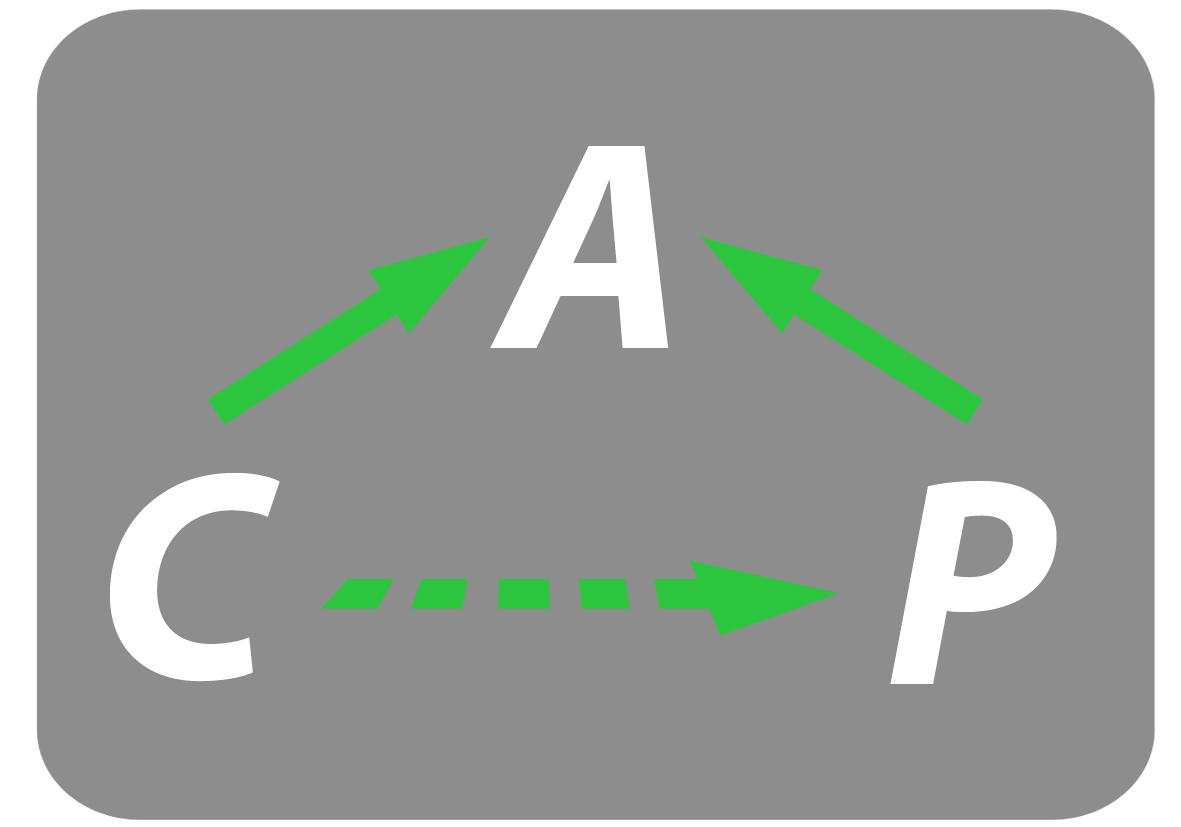
\includegraphics[width=0.25\textwidth,height=0.25\textheight]{Logo_CAP.jpg}}
\institute[Siegen]{University of Siegen}

\begin{document}

\defverbatim{\assemblyint}{
\begin{Verbatim}
addi:
movl  %edi, -4(%rsp)
movl  %esi, -8(%rsp)
movl  -4(%rsp), %esi
addl  -8(%rsp), %esi
movl  %esi, %eax
ret
\end{Verbatim}
}

\defverbatim{\cinteger}{
\begin{Verbatim}
int addi( int a,
	  int b )
{
  return a + b;
}
\end{Verbatim}
}

\defverbatim{\assemblyfloat}{
\begin{Verbatim}
addf:
movss %xmm0, -4(%rsp)
movss %xmm1, -8(%rsp)
movss -4(%rsp), %xmm0
addss -8(%rsp), %xmm0
ret
\end{Verbatim}
}

\defverbatim{\cfloat}{
\begin{Verbatim}
float addf( float a, 
	    float b )
{
  return a + b;
}
\end{Verbatim}
}

\defverbatim{\juliacode}{
\begin{Verbatim}
function( a, b )
    return a + b;
end;
\end{Verbatim}
}


\begin{frame}[fragile]
\titlepage
\end{frame}

% \begin{frame}
%  \frametitle{Outline}
%  \tableofcontents[pausesections]
% \end{frame}


%% Talk:
%% Posur: 1-4; 8-17; 24-35; 48-51
%% Gutsche: 5-7; 18-23; 36-47; 52-58

\part{Constructive category theory}


\tikzstyle{boxpackage} = [rectangle, rounded corners, minimum width=0.7cm, minimum height=0.6cm,text centered, draw=black, font=\footnotesize]

% Mathematics
\begin{frame}[fragile]
 \frametitle{Mathematics}
 \begin{block}{} 
  \begin{center}
   \begin{tikzpicture}[node distance=0.7cm, scale=0.5]
    \only<1-3>{
    \node (problem) [boxpackage, fill=\myblue] {Problem};
    }
    \visible<2->{
    \node (model) [boxpackage, below of=problem, yshift = -3em, fill=\myblue] {Mathematical context};
    }
    \only<2-3>{
    \draw[->,thick] (problem) --node[right]{Abstraction} (model);
    }
    \visible<3->{
    \node (solution) [boxpackage, below of=model,yshift = -3em, fill=\myblue] {Solution};    
    \draw[->,thick] (model) --node[right]{Methods} (solution);
    }
    \visible<4->{
    \node (problem1) [boxpackage, fill=\myblue] {Problem};
    \node (problem2) [boxpackage, fill=\myblue, left = of problem1] {Problem};
    \node (problem3) [boxpackage, fill=\myblue, right = of problem1] {Problem};
    \node (dotsleft) [left = of problem2] {$\dots$};
    \node (dotsright) [right = of problem3] {$\dots$};
    \draw[->,thick] (problem1) -- (model);
    \draw[->,thick] (problem2) -- (model);
    \draw[->,thick] (problem3) -- (model);
    \draw[->,thick] (dotsleft) -- (model);
    \draw[->,thick] (dotsright) -- (model);
    }
    \visible<5->{
    \draw[draw=none] (problem1) --node[]{$\simeq$} (problem2);
    \draw[draw=none] (problem3) --node[]{$\simeq$} (problem1);
    \draw[draw=none] (problem3) --node[]{$\simeq$} (dotsright);
    \draw[draw=none] (dotsleft) --node[]{$\simeq$} (problem2);
    }
    \end{tikzpicture}
  \end{center}
 \end{block}
\end{frame}

% Constructive category theory
\begin{frame}[fragile]
 \frametitle{Constructive category theory}
 \begin{block}{} 
  \begin{center}
   \begin{tikzpicture}[node distance=0.7cm, scale=0.6, every node/.style={scale=0.6}]
    \only<1-3>{
    \node (problem) [boxpackage, fill=\myblue] {Mathematical context};
    }
    \visible<2->{
    \node (model) [boxpackage, below of=problem, yshift = -3em, fill=\myblue] {Category};
    }
    \only<2>{
    \draw[->,thick] (problem) --node[right]{Abstraction} (model);
    }
    \visible<6->{
    \node (solution) [boxpackage, below of=model,yshift = -3em, fill=\myblue] {Solution};    
    \draw[->,thick] (model) --node[right]{Constructive category theory} (solution);
    }
    \visible<3->{
    \node (problem1) [boxpackage, fill=\myblue] {Mathematical context};
    \node (problem2) [boxpackage, fill=\myblue, left = of problem1] {Mathematical context};
    \node (problem3) [boxpackage, fill=\myblue, right = of problem1] {Mathematical context};
    \node (dotsleft) [left = of problem2] {$\dots$};
    \node (dotsright) [right = of problem3] {$\dots$};
    \draw[->,thick] (problem1) -- (model);
    \draw[->,thick] (problem2) -- (model);
    \draw[->,thick] (problem3) -- (model);
    \draw[->,thick] (dotsleft) -- (model);
    \draw[->,thick] (dotsright) -- (model);
    }
    \visible<4->{
    \draw[draw=none] (problem1) --node[]{$\simeq$} (problem2);
    \draw[draw=none] (problem3) --node[]{$\simeq$} (problem1);
    \draw[draw=none] (problem3) --node[]{$\simeq$} (dotsright);
    \draw[draw=none] (dotsleft) --node[]{$\simeq$} (problem2);
    }
    \visible<5->{
    \node (problem1n) [boxpackage, fill=\myblue, above = of problem1,xshift=+2.5em] {Problem};
    \node (problem2n) [boxpackage, fill=\myblue, above = of problem2,xshift=+2.5em] {Problem};
    \node (problem3n) [boxpackage, fill=\myblue, above = of problem3,xshift=+2.5em] {Problem};
    \node (problem1m) [boxpackage, fill=\myblue, above = of problem1,xshift=-2.5em] {Problem};
    \node (problem2m) [boxpackage, fill=\myblue, above = of problem2,xshift=-2.5em] {Problem};
    \node (problem3m) [boxpackage, fill=\myblue, above = of problem3,xshift=-2.5em] {Problem};
    \node (dotsleft) [left = of problem2m, xshift = +1em] {$\dots$};
    \node (dotsright) [right = of problem3n, xshift = -1em] {$\dots$};
%     
%     
    \draw[draw=none] (problem1n) --node[]{$\simeq$} (problem1m);
    \draw[draw=none] (problem2n) --node[]{$\simeq$} (problem2m);
    \draw[draw=none] (problem3n) --node[]{$\simeq$} (problem3m);
    
    \draw[draw=none] (problem2m) --node[]{$\simeq$} (problem1n);
    \draw[draw=none] (problem1m) --node[]{$\simeq$} (problem3n);
    \draw[draw=none] (problem2m) --node[]{$\simeq$} (dotsleft);
    \draw[draw=none] (problem3n) --node[]{$\simeq$} (dotsright);
    
    
    \draw[->,thick] (problem1n) -- (problem1);
    \draw[->,thick] (problem1m) -- (problem1);
    \draw[->,thick] (problem2n) -- (problem2);
    \draw[->,thick] (problem2m) -- (problem2);
    \draw[->,thick] (problem3n) -- (problem3);
    \draw[->,thick] (problem3m) -- (problem3);
    \draw[->,thick] (dotsleft) -- (problem2);
    \draw[->,thick] (dotsright) -- (problem3);
    
%     \draw[draw=none] (dotsrightn) --node[]{$\simeq$} (problem1n);
%     \draw[draw=none] (dotsrightn1) --node[]{$\simeq$} (problem3n);
%     \draw[draw=none] (dotsleftn1) --node[]{$\simeq$} (problem2n);
%     \draw[->,thick] (problem1n) -- (problem1);
%     \draw[->,thick] (problem2n) -- (problem2);
%     \draw[->,thick] (problem3n) -- (problem3);
    }
    \end{tikzpicture}
  \end{center}
 \end{block}
\end{frame}

% Abstraction of language
\begin{frame}[fragile]
 \frametitle{Abstraction of language}
 \pause
 \begin{block}{Addition of two numbers:\vphantom{AssemblyC\Gap or Julia} \only<3-5>{Assembly}\only<6-8>{C}\only<9->{\Gap or Julia}}
  \vspace*{-1.5em}
  \begin{overlayarea}{\linewidth}{12\baselineskip}

 \only<2-11>{
 \begin{columns}[onlytextwidth, t]
  \column{0.02\linewidth}
  
  \column{0.40\linewidth}
  \begin{block}{Data type: \texttt{int}}
  \begin{overlayarea}{\linewidth}{8\baselineskip}
\only<4-5>{
\vspace*{-1em}
\assemblyint
}
\only<7-8>{
 \cinteger
}
\only<10-11>{
 \juliacode
}
  \end{overlayarea}
  \end{block}
  \column{0.40\linewidth}
  \begin{block}{Data type: \texttt{float}}
  \begin{overlayarea}{\linewidth}{8\baselineskip}
\only<5>{
  \vspace*{-1em}
\assemblyfloat
}
\only<8>{
\cfloat
}
\only<11>{
 \juliacode
}
 \end{overlayarea}
 \end{block}
 \column{0.02\linewidth}
 \end{columns}
}
\only<12->{
 \begin{columns}
  \column{0.02\linewidth}
  
  \column{0.8\linewidth}
  \vspace{1.5em}
  \begin{block}{Data type: \texttt{int, float}}
  \juliacode
 \end{block}
 \begin{center}
  \visible<13->{High language leads to generic code!}
 \end{center}

 \column{0.02\linewidth}
 \end{columns}
}
 \end{overlayarea}
 \end{block}
\end{frame}

% Abstraction of language
\begin{frame}[fragile]
 \frametitle{Abstraction of language}
 \begin{block}{Computing the intersection of two subobjects}
  \begin{columns}[onlytextwidth, t]
  \column{0.02\linewidth}
  \column{0.40\linewidth}
  \pause
  \begin{block}{Vector spaces\vphantom{Ideals of $\mathbb{Z}$}}
  \begin{overlayarea}{\linewidth}{7\baselineskip}
  $\left\langle v_1, v_2 \right\rangle, \left\langle w_1, w_2 \right\rangle \leq V$:\newline \pause
  Solution of
  \begin{align*}
   & x_1v_1 + x_2 v_2 \\
   = & y_1w_1 +y_2w_2
  \end{align*}
  \end{overlayarea}
  \end{block} \pause
  \column{0.40\linewidth}
  \begin{block}{Ideals of $\mathbb{Z}$\vphantom{Vector spaces}} \pause
  \begin{overlayarea}{\linewidth}{7\baselineskip}
  $\left\langle x\right\rangle$, $\left\langle y\right\rangle \leq \Z:$\newline \pause
  Euclidean algorithm:
  \[
   \left\langle \mathrm{lcm} \left( x,y \right) \right\rangle
  \]
  
  \end{overlayarea}
  \end{block}\pause
  \column{0.02\linewidth}
  \end{columns}
 \begin{center}
 Generic algorithm for both cases? \pause
 \textbf{Category theory!}
 \end{center}
 \end{block}
\end{frame}

% Category theory as programming language
\begin{frame}
\frametitle{Category theory as programming language}
 \begin{block}{Category theory} \pause
 \begin{itemize}
  \item abstracts mathematical structures \pause
  \item defines a \textit{language} to formulate theorems and algorithms for different structures \textit{at the same time}\pause
 \end{itemize} 
 \end{block}
 \begin{block}{\CapPkg\ - Categories, Algorithms, Programming}
  \begin{columns}[onlytextwidth, t]
   \column{0.02\linewidth}
   \column{0.2\linewidth}
   \vspace{0.1em}
 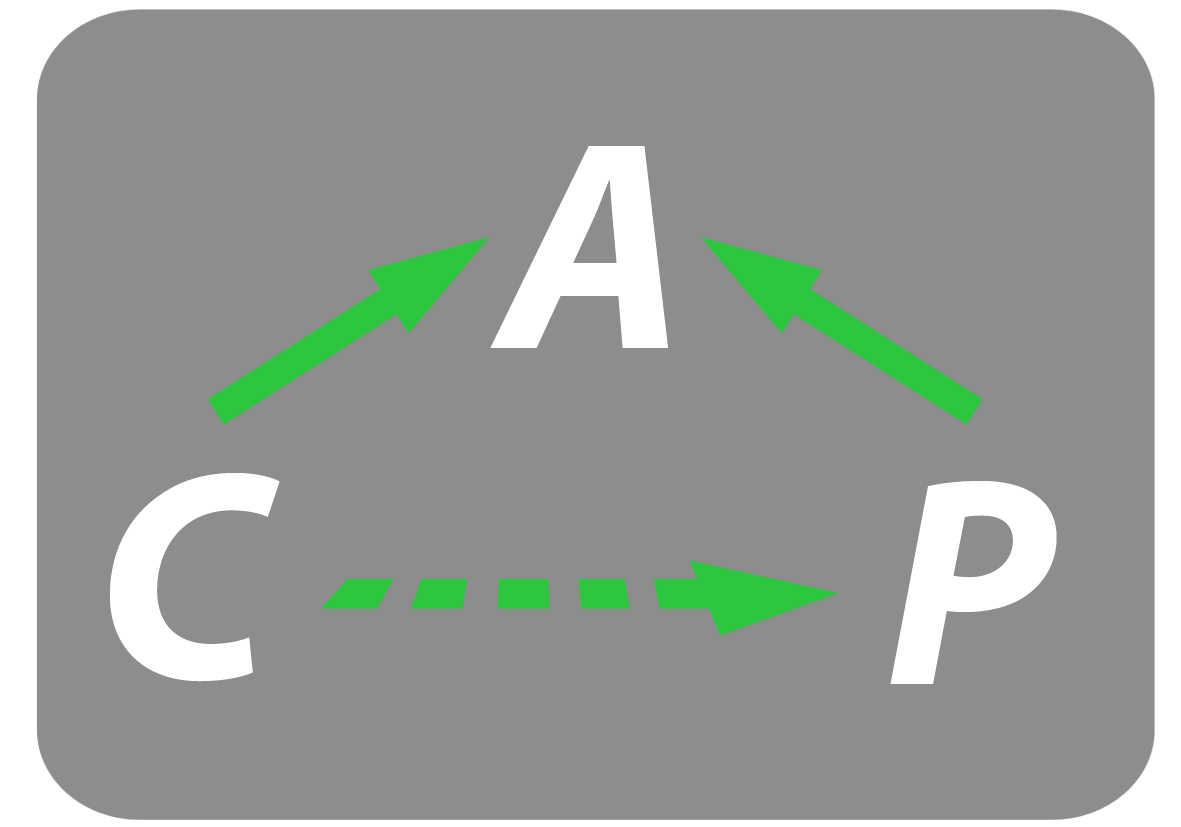
\includegraphics[width=\textwidth,height=0.8\textwidth]{Logo_CAPtrans.png} \pause
 \column{0.7\linewidth}
   \begin{center}
   \hspace{2em}\CapPkg implements a \newline \textbf{categorical programming language}
   \end{center}
  \column{0.02\linewidth}
  \end{columns}
 \end{block}
\end{frame}

% Categories
\begin{frame}[fragile]
 \frametitle{Categories}
 \begin{block}{Definition}
  A category $\mathcal{A}$ contains the following data:
  \pause
  \begin{itemize}
   \item $\Obj_\mathcal{A}$
   \visible<3->{
   \item $\Hom_\mathcal{A}( A, B )$}
   \visible<6->{
   \item $\circ: \Hom_\mathcal{A}( B,C ) \times \Hom_\mathcal{A}( A, B ) \rightarrow \Hom_\mathcal{A}( A, C )$ \visible<6->{{\small\ \ \ \ (assoc.)}} }
   \visible<8->{
   \item Neutral elements: $\id_A \in \Hom_\mathcal{A}( A, A )$}
  \end{itemize}
 \end{block}
 
 \begin{center}
      \begin{tikzpicture}[transform shape,mylabel/.style={thick, draw=black, align=center,minimum width=0.5cm, minimum height=0.5cm,fill=white}]
      \coordinate (r) at (3,0);
      \coordinate (d) at (0,-1);
      \visible<2->{
      \node (A) {\only<2>{\color{red}}$A$};
      \node (B) at ($(A) + (r)$) {\only<2>{\color{red}}$B$};
      \node (C) at ($(B) + (r)$) {\only<2>{\color{red}}$C$}; }
      \visible<4>{
      \path[->, thick, red] (A) edge (B);
      }
      \visible<5->{
      \path[->, thick] (A) edge (B);
      }
      \visible<5>{
      \path[->, thick,red] (B) edge (C);}
      \visible<6->{
      \path[->, thick] (B) edge (C);}
      \visible<7>{
      \draw[bend left,->,thick,out=35,in=145,red] (A) to (C);}
      \visible<8->{
      \draw[bend left,->,thick,out=35,in=145] (A) to (C);}
      \visible<9>{
      \draw[->,thick,red] (A) edge[looseness=5, out=240, in=  -60] (A);
      \draw[->,thick,red] (B) edge[looseness=5, out=240, in=  -60] (B);
      \draw[->,thick,red] (C) edge[looseness=5, out=240, in=  -60] (C);}
      \visible<10->{
      \draw[->,thick] (A) edge[looseness=5, out=240, in=  -60] (A);
      \draw[->,thick] (B) edge[looseness=5, out=240, in=  -60] (B);
      \draw[->,thick] (C) edge[looseness=5, out=240, in=  -60] (C);}
    \end{tikzpicture}
    \end{center}
\end{frame}

% $\kvec
\begin{frame}[fragile]
 \frametitle{Finite dimensional vector spaces}
 Let $k$ be a field (e.g., $k = \Q$).
 \pause
 \begin{block}{Example: $\kvec$}
  \begin{itemize}
   \item $\Obj := $ finite dimensional $k$-vector spaces
   \pause
   \item $\Hom(V,W) := $ $k$-linear maps $V \rightarrow W$
  \end{itemize}
 \end{block}
 
 \visible<6->{
 \begin{center}
    \scalebox{2}{${{\simeq}}$}
 \end{center}
 }
\pause
 \only<1-6>{
 \begin{block}{Example: matrices \phantom{(computerfriendly model)}}
  
  \begin{itemize}
   \item $\Obj := \N_0$
   \pause
   \item $\Hom(n,m) := k^{n\times m}$
  \end{itemize}
 \end{block}
 }
 \only<7->{
 \begin{block}{Example: matrices (computerfriendly model)}
  
  \begin{itemize}
   \item {\color{computerfriendly}$\Obj := \N_0$.}
   \pause
   \item {\color{computerfriendly}$\Hom(n,m) := k^{n\times m}$.}
  \end{itemize}
 \end{block}
 }
\end{frame}

% Computable categories
\begin{frame}[fragile]
 \frametitle{Computable categories}
 \pause
  A category becomes computable through\pause
  \begin{itemize}
   \item Data structures for \only<1-6,9->{\textit{objects}}\only<7-8>{{\color{red}\textit{objects}}} and \only<9-10>{{\color{red}\textit{morphisms}}}\only<1-8,11->{\textit{morphisms}} \pause
   \item Algorithms to compute the \only<1-10,13->{{\textit{composition}}}\only<11-12>{{\color{red}\textit{composition}}} of morphisms \pause
         and \only<1-12,15->{{\textit{identity morphisms}}}\only<13-14>{{\color{red}\textit{identity morphisms}}} of objects \pause
  \end{itemize}
 \begin{block}{Example: matrices}\pause
 \begin{center}
      \begin{tikzpicture}[transform shape,mylabel/.style={thick, draw=black, align=center,minimum width=0.5cm, minimum height=0.5cm,fill=white}]
      \coordinate (r) at (3,0);
      \coordinate (d) at (0,-1);
      \visible<9->{
      \node (A) {$1$};
      \node (B) at ($(A) + (r)$) {$2$};
      \node (C) at ($(B) + (r)$) {$1$}; }
      \visible<11->{
      \path[->, thick] (A) edge node[below]{$\left( \begin{array}{cc} 1 & 2 \end{array} \right)$} (B);
      }
      \visible<11->{
      \path[->, thick] (B) edge node[below]{$\left( \begin{array}{c} 3 \\ 4 \end{array} \right)$} (C);}
      \visible<13->{
      \path[bend left,->,thick,out=35,in=145] (A) edge node[above]{$\left( \begin{array}{cc} 1 & 2 \end{array} \right) \cdot \left( \begin{array}{c} 3 \\ 4 \end{array} \right) = \left( 11 \right)$} (C);}
      \visible<15->{
      \draw[->,thick] (A) edge[looseness=5, out=240, in=  -60] node[below] {{\small $(1)$}} (A);
      \draw[->,thick] (B) edge[looseness=5, out=240, in=  -60] node[below] {{\tiny $\left( \begin{array}{cc} 1 & 0 \\ 0 & 1 \end{array} \right)$}} (B);
      \draw[->,thick] (C) edge[looseness=5, out=240, in=  -60] node[below] {{\small $(1)$}} (C);}
      \visible<8>{
      \node[red] (A) {$1$};
      \node[red] (B) at ($(A) + (r)$) {$2$};
      \node[red] (C) at ($(B) + (r)$) {$1$}; }
      \visible<10>{
      \path[->, thick,red] (A) edge node[below,red]{$\left( \begin{array}{cc} 1 & 2 \end{array} \right)$} (B);
      }
      \visible<10>{
      \path[->, thick,red] (B) edge node[below,red]{$\left( \begin{array}{c} 3 \\ 4 \end{array} \right)$} (C);}
      \visible<12>{
      \path[bend left,->,thick,out=35,in=145,red] (A) edge node[above,red]{$\left( \begin{array}{cc} 1 & 2 \end{array} \right) \cdot\left( \begin{array}{c} 3 \\ 4 \end{array} \right) = \left( 11 \right)$} (C);}
      \visible<14>{
      \draw[->,thick,red] (A) edge[looseness=5, out=240, in=  -60] node[below] {{\small $(1)$}} (A);
      \draw[->,thick,red] (B) edge[looseness=5, out=240, in=  -60] node[below] {{\tiny $\left( \begin{array}{cc} 1 & 0 \\ 0 & 1 \end{array} \right)$}} (B);
      \draw[->,thick,red] (C) edge[looseness=5, out=240, in=  -60] node[below] {{\small $(1)$}} (C);}
    \end{tikzpicture}
    \end{center}
   \end{block}
\end{frame}

\begin{frame}[fragile]
  \frametitle{Finitely presented modules}
  Let $R$ be a ring, e.g., $R = \Z$.
  \begin{block}{Definition}
    $R$-modules of the form
    \[
      \frac{R^{1 \times n}}{\langle r_1, \dots, r_m \rangle}
    \]
    are called \textbf{finitely presented}, where $r_1, \dots, r_m \in R^{1 \times n}$.
  \end{block}
 \end{frame}
 
 \begin{frame}[fragile]
  \frametitle{Examples}
   $M \cong \frac{R^{1 \times n}}{\langle r_1, \dots, r_m \rangle}$
   \pause
   \begin{block}{$R =\Z$}
    \pause
    \[
     \frac{\Z}{\langle 2 \rangle}
    \]
    \pause
    \[
      \frac{\Z}{\langle 2 \rangle} \oplus \frac{\Z}{\langle 4 \rangle} \simeq \frac{\Z^{1 \times 2}}{\langle (2,0),(0,4) \rangle}
    \]
    \pause
    \[
    \frac{\Z^{1 \times 3}}{\scriptsize
    \langle
    \only<1-5>{
    \mathrm{Rows~of}
    }
    \left(
   \begin{array}{ccc}
    1 & 2 & 3 \\
    4 & 5 & 6 \\
    7 & 8 & 9 \\
   \end{array}
 \right)
 \rangle
 }
 \]
   \end{block}
  \pause
 \end{frame}

 \begin{frame}[fragile]
  \frametitle{Category of finitely presented modules}
  \begin{block}{}
  Finitely presented $R$-modules form a category
  \pause
  \[
  \modR 
  \]
  \pause
  with $R$-linear maps as morphisms.
  \end{block}
  \pause
  \begin{center}
   \textbf{\color{computerfriendly}{Computerfriendly model?}}
  \end{center}
 \end{frame}

\begin{frame}[fragile]
  \frametitle{Data structures: objects}
  
  \[
    \frac{\Z^{1 \times 3}}{\scriptsize
    \langle
    \only<1>{
    \mathrm{Rows~of}
    }
    \only<3->{
    \color{blue}
    }
    \left(
      \begin{array}{ccc}
        1 & 2 & 3 \\
        4 & 5 & 6 \\
        7 & 8 & 9 \\
       \end{array}
 \right)
 \rangle
 }
 \]
 \visible<4->{
 \begin{center}
 Idea: a matrix $M \in R^{m \times n}$ can represent the module $\frac{R^{1 \times n}}{\langle M \rangle}$. 
 \end{center}
 }
 \visible<5->{
 \begin{block}{Objects}
  \[
   \Obj_{\fpresR} := \biguplus_{m,n \in \N_0} R^{m \times n}
  \]
 \end{block}
 }
 
 \end{frame}

 
\begin{frame}[fragile]
 \frametitle{Data structures: morphisms}
 Given: $M \in R^{m \times n}$ and $M' \in R^{m' \times n'}$.
 \visible<2->{
 \begin{center}
  \begin{tikzpicture}
      \coordinate (r) at (3,0);
      \coordinate (d) at (0,-1);
      
      \node (M) {$\frac{R^{1 \times n}}{\langle M \rangle}$};
      \node (Mp) at ($(M) + (r)$) {$\frac{R^{1 \times n'}}{\langle M' \rangle}$};
      
      \visible<4->{
      \node (eM) at ($(M) + (d)$) {$\overline{e_i}$};
      }
      \visible<5->{
      \node (eMp) at ($(Mp) + (d)$) {$\overline{r_i}$};
      }
      
      \visible<3->{
      \draw[->,thick] (M) --node[above]{\text{\only<8->{$A :=$}\visible<6->{$\pmatcol{r_1}{\vdots}{r_n}$}}} (Mp);
      }
      \visible<5->{
      \draw[draw = none] (eM) --node[]{$\longmapsto$} (eMp);
      }
  \end{tikzpicture}
 \end{center}
 }
 \visible<7->{
\begin{block}{$\Hom_{\fpresR}( M, M' ) := $}
 \begin{center}
  \begin{minipage}{5em}
   \visible<8->{$A \in R^{n \times n'}\phantom{\big\{}$}
  \end{minipage}
  \begin{minipage}{5em}
   \visible<9->{such that}
  \end{minipage}
  \begin{minipage}{15em}
   \only<1-9>{\ }
   \only<10>{$\big\{ \text{Rows of~}M \cdot A \big\} \subseteq \langle M' \rangle$}
   \only<11->{\only<14>{\color{blue}}$\exists X \in R^{m \times m'}: M \cdot A = X \cdot M'\phantom{\big\{}$}
  \end{minipage}
 \end{center}
\end{block}
}
\visible<12->{
\begin{center}
 $A$ defines the $0$ morphism \visible<13->{iff {\only<14->{\color{blue}}$\exists X \in R^{n \times m'}: A = X \cdot M'$}}
\end{center}
}
\visible<15->{
  $\rightsquigarrow$ algorithmic requirements for $R$ \visible<16->{(for $R=\Z$, use Smith normal forms)}
}
\end{frame}



% The language of category theory
\begin{frame}[fragile]
  $\kvec$ and $\modZ$ are examples of \textbf{abelian categories}.
  \pause
 \frametitle{The language of category theory}
 \begin{block}{Some categorical operations in abelian categories}
  \begin{itemize}
   \pause
   \item $\oplus: \Obj \times \Obj \rightarrow \Obj$
   \pause
   \item $\circ: \Hom(B,C) \times \Hom(A,B) \rightarrow \Hom(A,C)$
   \pause
   \item $+,-: \Hom(A,B) \times \Hom(A,B) \rightarrow \Hom(A,B)$
   \pause
   \item {\only<8->{\color{red}}$\kernel: \Hom(A,B) \rightarrow \Obj$}
   \pause
   \item ...
  \end{itemize}
 \end{block}
\end{frame}

% Implementation of the kernel
\begin{frame}[fragile]
 \frametitle{Implementation of the kernel}
  Let $\varphi \in \Hom( A, B )$.
  \pause
  \visible<3->{To fully describe the kernel of $\varphi$ $\dots$}

\begin{block}{}
\begin{center}
   \visible<4->{$\dots$ one needs an object {\color{red}$\ker \phi$},\\}
   \visible<5->{its embedding {\color{red}  $\kappa = \KernelEmbedding( \phi )$},\\}
   \visible<6->{and for every test morphism $\tau$\\}
   \visible<7->{a \textit{unique} morphism {\color{red}$\lambda = \KernelLift( \phi, \tau )$}}\visible<8->{, such that}
\end{center}

\begin{center}
    \begin{tikzpicture}[label/.style={postaction={
      decorate,
      decoration={markings, mark=at position .5 with \node #1;}}}]
      \coordinate (r) at (1.5,0);
      \coordinate (u) at (0,0.75);
      
      \node (M) {$A$};
      \node (N) at ($(M)+(r)$) {$B$};
      \visible<4->{\node (K) at ($(M)-(r)+(u)$) {\color{red} $\ker \phi$};}
      \visible<6->{\node (L) at ($(K)-2*(u)$) {$T$};}
      \draw[->,thick] (M) -- node[above]{$\phi$} (N);
      \visible<6->{\draw[bend left,->,label={[above]{$0$}},thick] (K) to (N);}
      \visible<5->{\draw[red,right hook->,thick] (K) -- node[above]{\color{red} $\kappa$} (M);}
      \visible<6->{\draw[->,thick] (L) -- node[above]{$\tau$} (M);}
      \visible<6->{\draw[bend right,->,label={[below]{$0$}},thick] (L) to (N);}
      \visible<7->{\draw[red,->,dashed,thick] (L) -- node[left]{\color{red} $\lambda$} (K);}
      \visible<8->{\node (CC) at ($0.33*(L) + 0.33*(M) + 0.4*(K)$) {\small$\circlearrowright$};}
    \end{tikzpicture}
\end{center}
\end{block}
\end{frame}


% Implementation of the kernel: $\mathbb{Q}$-vector spaces
\begin{frame}[fragile]
 \frametitle{Implementation of the kernel: matrices}
 \begin{block}{}
  $\Obj := \N_{0}$, $\Hom \left( m, n \right) := \Q^{m \times n}$
 \end{block}
 \pause
 \begin{block}{}
  \begin{center}
   \begin{tikzpicture}[label/.style={postaction={
      decorate,
      decoration={markings, mark=at position .5 with \node #1;}}}]
      \coordinate (r) at (1.5,0);
      \coordinate (u) at (0,0.75);
      
      \node (M) {$A$};
      \node (N) at ($(M)+(r)$) {$B$};
      \visible<3->{\node (K) at ($(M)-(r)+(u)$) {\color{red} $\ker \phi$};}
      \visible<7->{\node (L) at ($(K)-2*(u)$) {$T$};}
      \draw[->,thick] (M) -- node[above]{$\phi$} (N);
      \visible<5->{\draw[red,right hook->,thick] (K) -- node[above]{\color{red} $\kappa$} (M);}
      \visible<7->{\draw[->,thick] (L) -- node[above]{$\tau$} (M);}
      \visible<8->{\draw[red,->,dashed,thick] (L) -- node[left]{\color{red} $\lambda$} (K);}
    \end{tikzpicture}
\end{center}
 \visible<4->{Compute}
 \begin{itemize}
  \visible<4->{\item $\ker \phi$ as $\mathrm{dim}(A) - \mathrm{rank}(\phi)$}
  \visible<6->{\item $\kappa$ by solving $X \cdot \phi = 0$}
  \visible<9->{\item $\lambda$ by solving $ X \cdot \kappa  = \tau$}
 \end{itemize}
 \end{block}
\end{frame}


% The language of category theory
\begin{frame}[fragile]
 \frametitle{The language of category theory}
 \pause
 \begin{overlayarea}{\linewidth}{\baselineskip}
  Given a diagram of abelian groups:
 \end{overlayarea}
 \pause
 \begin{block}{}
 \begin{overlayarea}{\linewidth}{5.3\baselineskip}
 \begin{center}
          \begin{tikzpicture}[transform shape,mylabel/.style={thick, draw=black, align=center, minimum width=0.5cm, minimum height=0.5cm,fill=white}]
            \matrix[matrix of nodes,column sep={70pt,between origins},row sep={40pt,between origins}] (s)
            { \phantom{$\in$}\vphantom{{$x\in A'$}} & |[name=Kap]| \vphantom{{$x\in A'$}}\vphantom{{$x \in {\color{blue}\Kernel}$}}\only<1-4>{\color{blue}$\Kernel$} \only<5-10>{$x \in {\color{blue}\Kernel}$} & |[name=Ap]| \only<1-5>{$A'$} \only<6->{$x\in A'$}\vphantom{{$x\in A'$}} & |[name=Bp]| $B'$ \vphantom{{$x\in A'$}}& \\
              \phantom{$y\in$} & |[name=Ka]| \vphantom{{$\alpha(x)\in A$}}\only<1-8>{\color{computerfriendly}$\Kernel$} \only<9->{$\alpha(x) \in {\color{computerfriendly}\Kernel}$} & |[name=A]| \only<1-6>{$A$} \only<7->{$\alpha(x)\in A$} \vphantom{{$\alpha(x)\in A$}}& |[name=B]| \only<1-7>{$B$} \only<8->{$0 \in B$} \vphantom{{$\alpha(x)\in A$}}& \\
            };
            \path[right hook->,thick] (Kap) edge node[above]{$\phantom{\kappa'}$}(Ap);
            \path[->,thick,blue] (Ap) edge (Bp);
            \path[right hook->,thick] (Ka) edge (A);
            \path[->,thick,computerfriendly] (A) edge (B);
            
            \path[->, thick] (Ap) edge node[left]{$\alpha$} (A);
            \path[->, thick] (Bp) edge (B);
            \only<4->{
            \path[->, thick, dashed] (Kap) edge (Ka);
            }
%             \only<10->{
%             \draw[->, thick, draw=none] ($(Kap) + (-0.45,-0.3)$) --node[rotate=270]{$\mapsto$} ($(Ka) + (-0.45,0.3)$);
%             }
          \end{tikzpicture}
  \end{center}
 \end{overlayarea}
  \end{block}
  \pause
  \begin{overlayarea}{\linewidth}{2\baselineskip} 
  \begin{center}
  \phantom{{{$\dashdownarrow$}} { $=$} {$\KernelLift( \phi, $}{$\alpha \circ \kappa'$}{$)$}} 
  \end{center}
  \end{overlayarea}
\end{frame}

% The language of category theory
\begin{frame}[fragile]
\frametitle{The language of category theory}
\begin{overlayarea}{\linewidth}{\baselineskip}
The same example in the language of category theory:
\end{overlayarea}
\begin{block}{}
\begin{overlayarea}{\linewidth}{5.3\baselineskip} 
 \begin{center}
          \begin{tikzpicture}[transform shape,mylabel/.style={thick, draw=black, align=center, minimum width=0.5cm, minimum height=0.5cm,fill=white}]
            \matrix[matrix of nodes,column sep={70pt,between origins},row sep={40pt,between origins}] (s)
            { \phantom{$\in$} & |[name=Kap]| \vphantom{$\Kernel A' B'$}{\color{blue}$\Kernel$} & |[name=Ap]| \vphantom{$\Kernel A' B'$}$A'$ & |[name=Bp]| \vphantom{$\Kernel A' B'$}$B'$ & \\
              \phantom{$\in$} & |[name=Ka]| \vphantom{$A B \Kernel$}{\color{computerfriendly}$\Kernel$}  & |[name=A]| \vphantom{$A B \Kernel$}{$A$}  & |[name=B]| \vphantom{$A B \Kernel$}{$B$}  & \\
            };
            \path[->,thick] (Kap) edge node[above]{$\kappa'$} (Ap);
            \path[->,thick,blue] (Ap) edge (Bp);
            \path[->,thick] (Ka) edge (A);
            \path[->,thick,computerfriendly] (A) edge node[above]{$\phi$}(B);     
            \path[->, thick] (Ap) edge node[left]{$\alpha$} (A);
            \path[->, thick] (Bp) edge (B);
            \path[->, thick, dashed] (Kap) edge (Ka);
            \visible<4->{
            \path[->,thick,red] (Kap) edge (A);}
          \end{tikzpicture}
  \end{center}
\end{overlayarea}
  \end{block}
  \begin{overlayarea}{\linewidth}{2\baselineskip}
  \begin{center}
    \visible<2->{{$\dashdownarrow$}} \visible<3->{ $=$} \visible<5->{$\KernelLift( {\color{computerfriendly}\phi}, $}\visible<4->{{\color{red}$\alpha \circ \kappa'$}}\visible<5->{$)$}
  \end{center}
  \end{overlayarea}
\end{frame}


% What is \CapPkg?
\begin{frame}
\frametitle{Features of \CapPkg}

\begin{block}{\CapPkg\ - Categories, Algorithms, Programming}
 \pause
  \CapPkg is a framework to implement computable categories and provides \pause
  \begin{itemize}
   \item specifications of categorical operations, \pause
   \item generic algorithms based on basic categorical operations,  \pause
   \item a categorical programming language having categorical operations as syntax elements
 \end{itemize}
\end{block}
\end{frame}

% Computing the intersection
\begin{frame}[fragile]
 \frametitle{Computing the intersection}
 Let $M_1 \only<1>{\subseteq}\only<2->{{\only<2>{\color{red}}\hookrightarrow}\ }N$ and $M_2 \only<1>{\subseteq}\only<2->{{\only<2>{\color{red}}\hookrightarrow}\ }N$ subobjects in an abelian category. \newline \pause \pause
   Compute their intersection $\gamma: M_1 \cap M_2 \hookrightarrow N$.
 \begin{block}{}
 \begin{center}
   \begin{tikzpicture}[label/.style={postaction={
      decorate,
      decoration={markings, mark=at position .5 with \node #1;}}}]
      \coordinate (r) at (2.7,0);
      \coordinate (u) at (0,1.5);
      
      \visible<11-12>{\node (M12) {$M_1 \cap M_2$};}
      \visible<5->{\node (M1p2) at ($(M12)+(r)$) {$M_1 \oplus M_2$};}
      \visible<4->{
      \node (M1) at ($(M1p2)+(r)+(u)$) {$M_1$};
      \node (M2) at ($(M1p2)+(r)-(u)$) {$M_2$};
      }
      \visible<4-12>{\node (N) at ($(M1p2)+2*(r)$) {$N$};}
      
      \visible<4->{
          \path[right hook->,thick] (M2) edge node[below]{$\iota_2$} (N);
      }
      \visible<4-12>{
          \path[right hook->,thick] (M1) edge node[above]{$\iota_1$} (N);
      }
      \visible<6-12>{
          \path[->>,thick] (M1p2) edge node[above]{$\pi_1$} (M1);
      }
      \visible<7->{
          \path[->>,thick] (M1p2) edge node[below]{$\pi_2$} (M2);
      }
      
      \visible<9->{
          \path[->,thick] (M1p2) edge node[above]{$\phi := \iota_1 \circ \pi_1 -  \iota_2 \circ \pi_2$} (N);
      }
      \visible<11-12>{
          \path[right hook->,thick] (M12) edge node[above]{$\kappa$} (M1p2);
      }
      \visible<13->{
          \path[right hook->,color=red,thick] (M12) edge node[above]{$\kappa$} (M1p2);
          \path[->>,color=red,thick] (M1p2) edge node[above]{$\pi_1$} (M1);
          \path[right hook->,color=red,thick] (M1) edge node[above]{$\iota_1$} (N);
          \node[color=red,thick] at ($(M12)$) {$M_1 \cap M_2$};
          \node[color=red,thick] at ($(N)$) {$N$};
     }
    \end{tikzpicture}
\end{center}
 \end{block}
 \begin{itemize}
  \visible<8->{ \item $\pi_i := \mathrm{ProjectionInFactorOfDirectSum}\left( \left( M_1, M_2 \right), i \right)$, $i=1,2$ }
%   \visible<9->{ \item $\pi_2 := \mathrm{ProjectionInFactorOfDirectSum}\left( \left( M_1, M_2 \right), 2 \right)$ }
  \visible<10->{ \item $\phi := \iota_1 \circ \pi_1 - \iota_2 \circ \pi_2$ }
  \visible<12->{ \item $\kappa := \mathrm{KernelEmbedding} \left( \phi \right)$ }
  \visible<14->{ \item $\gamma := \iota_1 \circ \pi_1 \circ \kappa$ } 
 \end{itemize}
\end{frame}

\defverbatim{\translationone}{
\begin{Verbatim}[fontsize=\small,commandchars=\\\{\}]
  pi1 := ProjectionInFactorOfDirectSum( [ M1, M2 ], 1 );
  pi2 := ProjectionInFactorOfDirectSum( [ M1, M2 ], 2 );
\end{Verbatim}
}


\defverbatim{\translationthree}{
\begin{Verbatim}[fontsize=\small,commandchars=\\\{\}]
  lambda := PostCompose( iota1, pi1 );
  phi := lambda - PostCompose( iota2, pi2 );
\end{Verbatim}
}

\defverbatim{\translationfour}{
\begin{Verbatim}[fontsize=\small,commandchars=\\\{\}]
  kappa := KernelEmbedding( phi );
\end{Verbatim}
}

\defverbatim{\translationfive}{
\begin{Verbatim}[fontsize=\small,commandchars=\\\{\}]
  gamma := PostCompose( lambda, kappa );
\end{Verbatim}
}

\defverbatim{\headerofintersection}{
\begin{Verbatim}[fontsize=\small,commandchars=\\\{\}]
IntersectionOfSubobject := function( iota1, iota2 )
\end{Verbatim}
}

\defverbatim{\localsofintersection}{
\begin{Verbatim}[fontsize=\small,commandchars=\\\{\}]
  local M1, M2, pi1, pi2, lambda, phi, kappa, gamma;
\end{Verbatim}
}

\defverbatim{\sourcesofintersection}{
\begin{Verbatim}[fontsize=\small,commandchars=\\\{\}]
  M1 := Source( iota1 );
  M2 := Source( iota2 );
\end{Verbatim}
}

\defverbatim{\footerofintersection}{
\begin{Verbatim}[fontsize=\small,commandchars=\\\{\}]
  return gamma;
end;
\end{Verbatim}
}

% Translation to \CapPkg
\begin{frame}[fragile]
 \frametitle{Translation to \CapPkg}
  \begin{overlayarea}{\linewidth}{14\baselineskip}
  \only<1-6>{\visible<1-5>{$\pi_i := \mathrm{ProjectionInFactorOfDirectSum}\left( \left( M_1, M_2 \right), i \right)$, $i=1,2$}}
  \only<7->{
  \visible<8->{
  \headerofintersection
  }
  \visible<11->{
  \localsofintersection
  }
  \visible<9->{
  \sourcesofintersection
  }
  }
  \visible<2->{{\color{red}\translationone}}
  \only<1-6>{\visible<1-5>{$\phi := \iota_1 \circ \pi_1 - \iota_2 \circ \pi_2$}}
  \visible<3->{{\color{red}\translationthree}}
  \only<1-6>{\visible<1-5>{$\kappa := \mathrm{KernelEmbedding} \left( \phi \right)$}}
  \visible<4->{{\color{red}\translationfour}}
  \only<1-6>{\visible<1-5>{$\gamma := \iota_1 \circ \pi_1 \circ \kappa$}}
  \visible<5->{{\color{red}\translationfive}}
  \only<7->{
  \visible<10->{
  \footerofintersection
  }}
  \end{overlayarea}
 \pause \pause \pause \pause \pause \pause \pause \pause
\end{frame}

% Computing the intersection: $\mathbb{Q}$-vector space
\begin{frame}[fragile]
 \frametitle{Computing the intersection: $\Q\mathrm{\text{-}vec}$}
 Compute the intersection of
\begin{center}
  \begin{tikzpicture}[label/.style={postaction={
      decorate,
      decoration={markings, mark=at position .5 with \node #1;}}}]
      \coordinate (r) at (1.5,0);
      \coordinate (u) at (0,0.75);
      
      \node (N) {$N$};
      \node (M1) at ($(N)-3*(r)$) {$M_1$};
      \node (M2) at ($(N)+3*(r)$)  {$M_2$};
      
      \node (Nn) at ($(N)-0.95*(u)$) {$3$};
      \node (M1n) at ($(M1)-0.95*(u)$) {$2$};
      \node (M2n) at ($(M2)-0.95*(u)$) {$2$};
      
      \draw[double equal sign distance] (Nn) to (N);
      \draw[double equal sign distance] (M1n) to (M1);
      \draw[double equal sign distance] (M2n) to (M2);
      
      \path[right hook->,thick] (M1) edge node[above] {\small $\iota_1 := \left( \begin{array}{ccc} 1 & 1 & 0 \\ 0 & 1 & 1 \end{array} \right)$} (N);
      \path[left hook->,thick] (M2) edge node[above] {\small $\iota_2 := \left( \begin{array}{ccc} 1 & 0 & 1 \\ 1 & 1 & 0 \end{array} \right)$} (N);
    \end{tikzpicture}
\end{center}
\pause
\begin{Verbatim}[commandchars=!@\%,fontsize=\small]
!color@blue%@gap>%!color@red%@ gamma := IntersectionOfSubobject( iota1, iota2 );%
<A morphism in the category of matrices over Q>
\end{Verbatim}
\pause
\begin{Verbatim}[commandchars=!@\%,fontsize=\small]
!color@blue%@gap>%!color@red%@ Display( gamma );%
[ [  1,  1,  0 ] ]

A morphism in the category of matrices over Q
\end{Verbatim}
\end{frame}


\tikzstyle{boxpackage} = [rectangle, rounded corners, minimum width=0.7cm, minimum height=0.6cm,text centered, draw=black, font=\footnotesize]

%%%% \CapPkg Pakete
\begin{frame}[fragile]
 \frametitle{\CapPkg packages}
%  \tikz[remember picture,overlay] \node[opacity=0.3,inner sep=0pt] at (current block.center){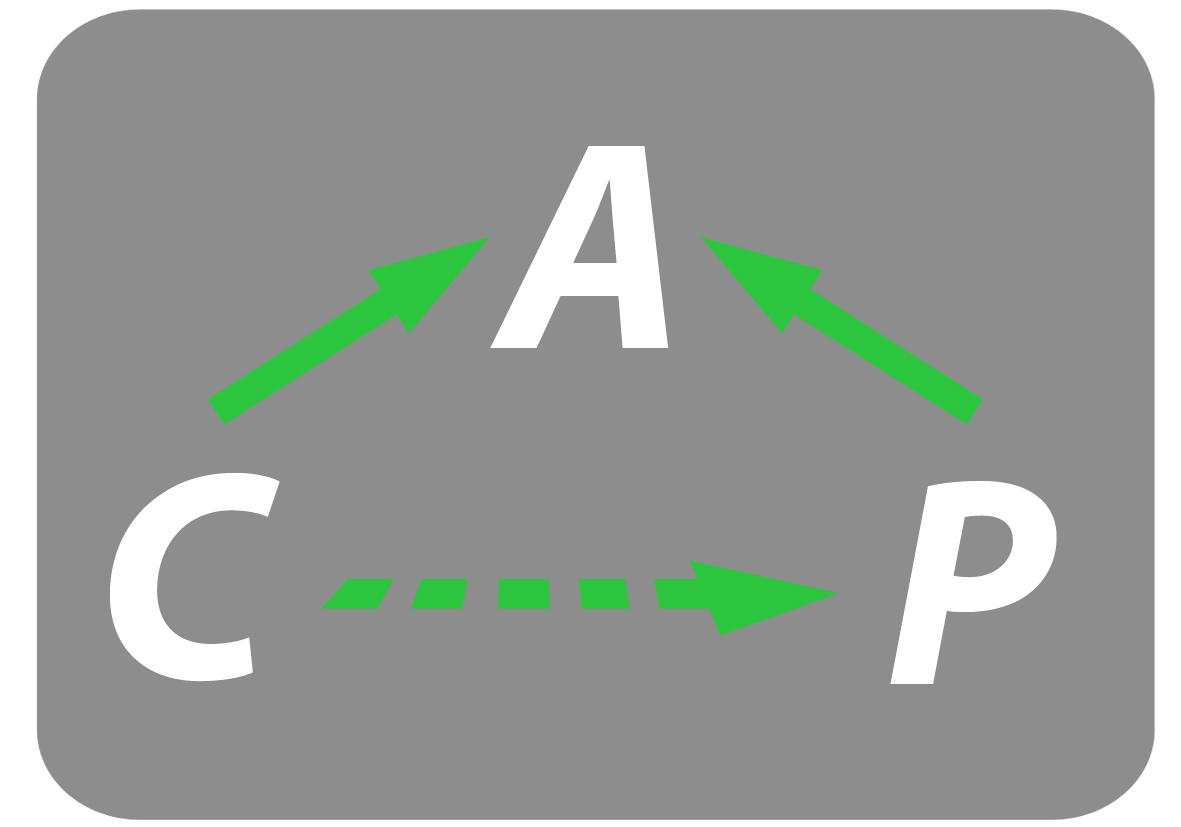
\includegraphics[width=\blockwidth,height=\blockheight]{Logo_CAP.jpg}};
  \begin{center}
   \begin{tikzpicture}[node distance=0.7cm,scale=0.6, every node/.style={scale=0.6}]
    {
    \node (intrinsic)[boxpackage, fill=\myblue] {IntrinsicCategories};
    }
    {
    \node (attribute)[boxpackage, fill=\myblue, below of= intrinsic] {AttributeCategory};
    \node (linearalgebra) [boxpackage, below of=attribute, fill=\myblue] {LinearAlgebra};
    \node (complexes) [boxpackage, below of=linearalgebra, fill=\myblue] {ComplexesAndFilteredObjects};
    \node (genmor) [boxpackage, below of=complexes, fill=\myblue] {GeneralizedMorphisms};
    \node (modulepres) [boxpackage, below of=genmor, fill=\myblue] {ModulePresentations};
    \node (homalg) [boxpackage, right = of genmor, fill=\myblue] {HomologicalAlgebra};
    \draw[->,thick] (homalg) |- (complexes);
    \draw[->,thick] (homalg.west) |- (genmor);
    }
    {
    \node (cap) [below = of modulepres] {};
    \begin{scope}[on background layer]
    \node (captotal) at ($(cap)+(1,0)$) [opacity=.20] {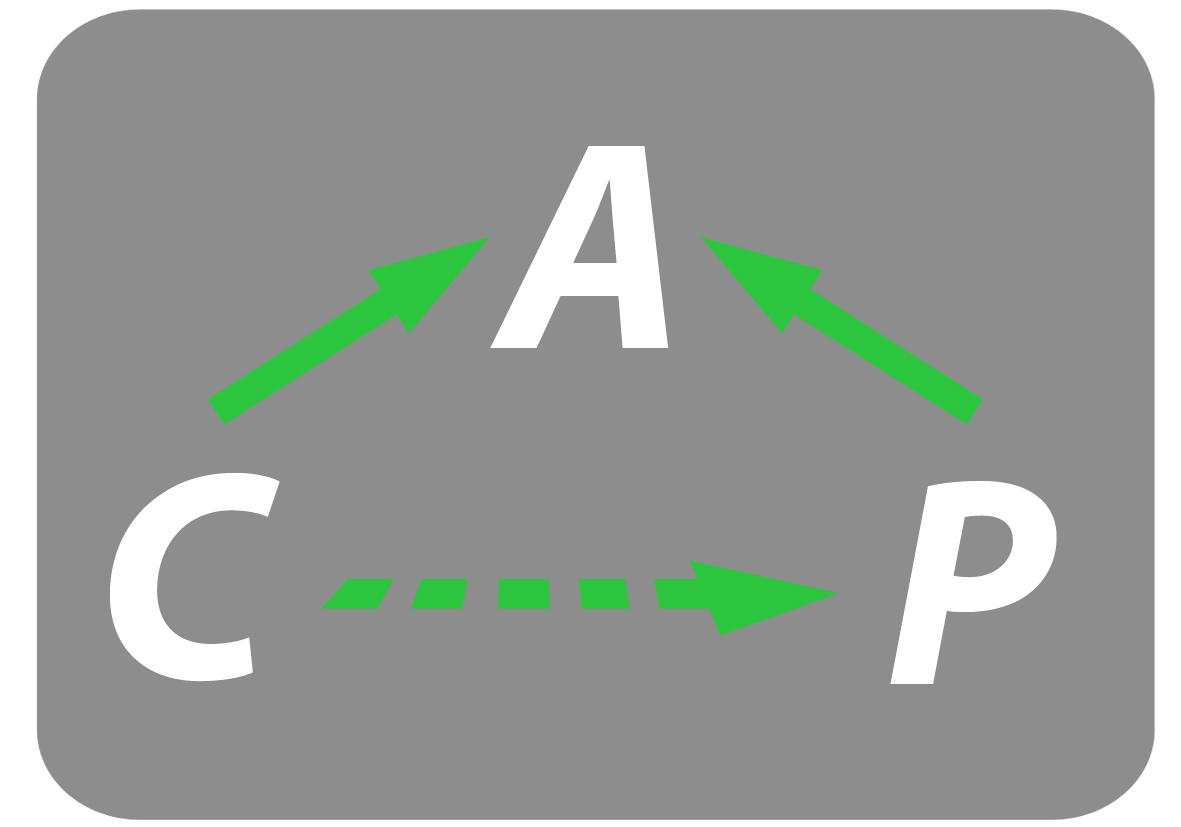
\includegraphics[width=1.4\textwidth]{Logo_CAP.jpg}};
    \end{scope}
    }
    
    {
    \node (ambient) [boxpackage, left = of attribute, fill=\myblue, xshift = -3em] {CategoriesWithAmbientObjects};
    \node (m2) [boxpackage, below = of ambient, fill=\myblue] {homalg2};
    \draw[->,thick] (m2) -- (ambient);
    \draw[->,thick] (m2) |- (modulepres);
    \draw[->,thick] (ambient) -- (attribute);
    }
    
    {
    \node (kamalcomplexes) [boxpackage, left = of cap, fill=\myblue, yshift = -4em] {complex};
    \node (stable) [boxpackage, below of=  kamalcomplexes, fill=\myblue] {StableCategories};
    \node (frobenius) [boxpackage, below of= stable, fill=\myblue] {FrobeniusCategories};
    \node (triangulated) [boxpackage, below of= frobenius, fill=\myblue] {TriangulatedCategories};
    \node (bicomplexes) [boxpackage, left= of kamalcomplexes, fill=\myblue] {Bicomplexes};
    \node (homotopy) [boxpackage, above= of bicomplexes, fill=\myblue, yshift = -2em, xshift = -1em] {HomotopyCategories};
    \draw[->,thick] (bicomplexes) -- (kamalcomplexes);
    \draw[->,thick] (homotopy.east) |- (kamalcomplexes);
    }
    
    {
    \node (qpa2) [boxpackage, right= of triangulated, fill=\myblue] {QPA2};
    }
    
    {
    \node (projectivegraded) [boxpackage, right = of cap, fill=\myblue, yshift = -4em] {CategoryOfProjectiveGradedObjects};
    \node (prescat) [boxpackage, below of = projectivegraded, fill=\myblue] {PresentationCategory};
    \node (presbyprojgraded) [boxpackage, below of = prescat, fill=\myblue, xshift = 8em] {PresentationsByProjectiveGradedModules};
    \draw[->,thick] (presbyprojgraded) |- (projectivegraded);
    \draw[->,thick] (presbyprojgraded) |- (prescat);
    }
    {
    \node (motives) [boxpackage, below = of m2, fill=\myblue, xshift = -3em] {MotivesForBiArrangements};
        }
    {
    \node (dmod) [boxpackage, right = of qpa2, fill=\myblue] {Bialgebroids};
    \draw[->,thick] (dmod) -- (qpa2);
    \node (functorcat) [boxpackage, below = of dmod, fill=\myblue] {FunctorCategories};
    \draw[->,thick] (functorcat) -- (dmod);
%     \node (bmod) [boxpackage, left = of functorcat, fill=\myblue,xshift=-1em] {BMod};
    }
    {
    \node (freydcats) [boxpackage, right = of dmod, fill=\myblue, yshift = -3em] {FreydCategories};
    \draw[->,thick] (freydcats) |- (dmod);
    }
    
    {
    \node (gradedmod) [boxpackage, right = of modulepres, fill=\myblue] {GradedModulePresentations};
    \node (toricsheaves) [boxpackage, below = of gradedmod, fill=\myblue] {ToricSheaves};
    \draw[->,thick] (gradedmod) -- (modulepres);
    \draw[->,thick] (toricsheaves) -- (gradedmod);
    }
    {
    \node (actions) [boxpackage, right = of attribute, fill=\myblue] {Actions};
    \node (groups) [boxpackage, right = of linearalgebra, fill=\myblue] {GroupRepresentations};
    \node (intext) [boxpackage, right = of groups, fill=\myblue] {InternalExteriorAlgebra};
    \draw[->,thick] (actions) -- (attribute);
    \draw[->,thick] (groups) -- (linearalgebra);
    \draw[->,thick] (intext) -- (groups);
    \draw[->,thick] (intext) |- (actions);
    \draw[->,thick] (intext) |- (complexes);
    }
    
    
    \end{tikzpicture}
  \end{center}
\end{frame}


% Connecting Homomorphism in the Snake Lemma

\begin{frame}[fragile]
 \frametitle{Snake lemma}

 \begin{block}{}
 \begin{center}
 \begin{tikzpicture}[mystyle/.style={scale=.7}]
  \matrix[matrix of math nodes,column sep={70pt,between origins},row sep={40pt,between origins}] (s)
  { & & & |[name=Kernel]| \kernel(\gamma) & \\
    &|[name=A]| A &|[name=B]| B &|[name=C]| C &|[name=01]| 0 \phantom{C}  \\
    |[name=02]| \phantom{a'} 0 &|[name=A']| A' &|[name=B']| B' &|[name=C']| C' \\
    & |[name=Coker]| \coker(\alpha) & & & \\
  };
              {\path[->,thick] (Kernel) edge node[mystyle,anchor=west] {} (C); }
              
              
              \path[->,thick] (C) edge (01);
              \path[->,thick] (A) edge (B);
              
              {\path[->,thick] (B) edge node[mystyle,anchor=south] {$\epsilon$} (C);}
              
              \path[->,thick] (A) edge node[mystyle,anchor=east] {$\alpha$} (A');
              
              {\path[->,thick] (B) edge node[mystyle, anchor=east] {$\beta$} (B');}
              
              \path[->,thick] (C) edge node[mystyle,anchor=east] {$\gamma$} (C');
              \path[->,thick] (02) edge (A');
              
              {\path[->,thick] (A') edge node[mystyle,anchor=north] {$\mu$} (B');}
              
              \path[->,thick] (B') edge (C');
              
              {\path[->,thick] (A') edge node[mystyle,anchor=east] {}(Coker);}
              \visible<2->{
              \draw[->,blue,rounded corners,thick] (Kernel) -| ($(01.east)+(.5,0)$) |- ($(B)!.35!(B')$) -|
    ($(02.west)+(-.5,0)$) |- (Coker);}
  \end{tikzpicture}
 \end{center}
 \end{block}
\end{frame}


\part{Generalized morphisms}

\begin{frame}
 \frametitle{}
 \tableofcontents
\end{frame}

\section{Classical diagram chases}


% What are diagram chases?
\begin{frame}[fragile]
 \frametitle{What are diagram chases?}
 \pause
 \begin{block}{}
  Diagram chases are a tool in homological algebra
  used for proving 
  \pause
  \begin{enumerate}
   \item properties
   \pause
   \item {\only<7->{\color{red}}the existence}
   \pause
  \end{enumerate}
  of morphisms 
  \pause
  situated in (commutative) diagrams of prescribed shape.
 \end{block}
\end{frame}

% Connecting homomorphism in the snake lemma
\begin{frame}[fragile]
 \frametitle{Connecting homomorphism in the snake lemma}
 \begin{center}
 \begin{tikzpicture}[mystyle/.style={scale=.7}]
  \matrix[matrix of math nodes,column sep={70pt,between origins},row sep={40pt,between origins}] (s)
  { & & & |[name=Kernel]| \text{\only<1>{$\kernel(\gamma)$}\only<2>{${\color{red}c} \in \kernel(\gamma)$}\only<3->{$c \in \kernel(\gamma)$ }} & \\
    &|[name=A]| A &|[name=B]| \text{\only<1-3>{$B$}\only<4>{${\color{red}b} \in B$}\only<5->{$b \in B$}} &|[name=C]| \text{\only<1-2>{$\coker\delta$}\only<3>{${\color{red}c} \in \coker\delta$}\only<4->{$c \in \coker\delta$}} &|[name=01]| 0 \phantom{C}  \\
    |[name=02]| \phantom{a'} 0 &|[name=A']| \text{ \only<1-5>{$\ker\lambda$}\only<6>{${\color{red}a'} \in \ker\lambda$}\only<7->{$a' \in \ker\lambda$} } &|[name=B']| \text{ \only<1-4>{$B'$}\only<5>{${\color{red}b'} \in B'$}\only<6->{$b' \in B'$} } &|[name=C']| C' \\
    & |[name=Coker]| \text{ \only<1-6>{$\coker(\alpha)$}\only<7>{${\color{red}a' + \im( \alpha )}\in \coker( \alpha )$}\only<8->{$a' + \im( \alpha )\in \coker( \alpha )$} } & & & \\
  };
              \path[->,thick] (Kernel) edge (C);
              \path[->,thick] (C) edge (01);
              \path[->,thick] (A) edge node[mystyle,anchor=south]{$\delta$} (B);
              \path[->,thick] (B) edge node[mystyle,anchor=south] {$\epsilon$} (C);
              \path[->,thick] (A) edge node[mystyle,anchor=east] {$\alpha$} (A');
              \path[->,thick] (B) edge node[mystyle, anchor=east] {$\beta$} (B');
              \path[->,thick] (C) edge node[mystyle,anchor=east] {$\gamma$} (C');
              \path[->,thick] (02) edge (A');
              \path[->,thick] (A') edge node[mystyle,anchor=north] {$\mu$} (B');
              \path[->,thick] (B') edge node[mystyle,anchor=south]{$\lambda$} (C');
              \path[->,thick] (A') edge (Coker);
              \visible<8->{
              \draw[->,rounded corners,thick,blue] (Kernel) -| ($(01.east)+(.5,0)$) |- ($(B)!.35!(B')$) -|
    ($(02.west)+(-.5,0)$) |- (Coker);}
  \end{tikzpicture}
 \end{center}
 
 \begin{block}{}
 \begin{center}
  \only<1>{Wanted: $\kernel(\gamma) \stackrel{\partial}{\longrightarrow} \coker( \alpha )$. \phantom{$\stackrel{:}{T_g}$} }
  \only<2>{Start: $c \in \kernel( \gamma )$. \phantom{$\stackrel{:}{T_g}$}}
  \only<3>{This lies in $\coker\delta$. \phantom{$\stackrel{:}{T_g}$}}
  \only<4>{Choose: $b \in \epsilon^{-1}(\{c\})$. \phantom{$\stackrel{:}{T_g}$}}
  \only<5>{Map: $b \stackrel{\beta}{\mapsto} b'$. \phantom{$\stackrel{:}{T_g}$} }
  \only<6>{Compute: $a' \in \mu^{-1}(b')$. \phantom{$\stackrel{:}{T_g}$} }
  \only<7>{Map: $a' \mapsto a' + \im( \alpha )$.\phantom{$\stackrel{:}{T_g}$}}
  \only<8-9>{ Result: $c \stackrel{{\color{blue}\partial}}{\mapsto} a' + \im( \alpha )$.
  \visible<9>{\textbf{Context}: modules} \phantom{$\stackrel{:}{T_g}$}}
  \end{center}
 \end{block}
\end{frame}


% Classical solutions: embedding theorems
\begin{frame}[fragile]
\frametitle{Classical solutions: embedding theorems}
 \pause
 \begin{block}{Freyd-Mitchell embedding theorem}
  \pause
  Any small abelian category $\mathbf{A}$ admits an exact fully faithful covariant embedding 
  \[
   F: \mathbf{A} \hookrightarrow R-\mathbf{mod}
  \]
  into the category of $R$-modules for some ring $R$.
 \end{block}
 \pause
 \begin{block}{Application: existence of morphisms}
  \begin{center}
   \begin{tikzpicture}
   \coordinate (r) at (4,0);
   \coordinate (d) at (0,-1);
   \node (A) {$\Hom_{\mathbf{A}}(A,B)$};
   \node (B) at ($(A) + (r)$) {$\Hom_{R-\mathbf{mod}}(FA,FB)$};
   \visible<6->{
   \node (a) at ($(A) + (d)$) {$F^{-1}\phi$};
   }
   \visible<5->{
   \node (b) at ($(B) + (d)$) {$\phi$};
   }
   
   \draw[draw=none] (A) -- node[]{$\cong$} (B);
   \visible<6->{
   \draw[draw=none] (a) -- node[rotate=90]{$\in$} (A);
   \draw[draw=none] (a) -- node[]{$\leftrightarrow$} (b);
   }
   \visible<5->{
   \draw[draw=none] (b) -- node[rotate=90]{$\in$} (B);
   }
  \end{tikzpicture}
  \end{center}
 \end{block}
 \visible<7->{
  Problem: this isomorphism between $\Hom$-sets is \textbf{not constructive}.
  }
\end{frame}


\section{Additive relations}

% Back to the snake lemma
\begin{frame}[fragile]
 \frametitle{Back to the snake lemma}
 \begin{center}
 \begin{tikzpicture}[mystyle/.style={scale=.7}]
  \matrix[matrix of math nodes,column sep={70pt,between origins},row sep={40pt,between origins}] (s)
  { & & & |[name=Kernel]| \text{{$c \in \kernel(\gamma)$ }} & \\
    &|[name=A]| A &|[name=B]| \text{{\only<2->{\color{red}}$b \in B$}} &|[name=C]| \text{{$c \in \coker\delta$}} &|[name=01]| 0 \phantom{C}  \\
    |[name=02]| \phantom{a'} 0 &|[name=A']| \text{ {$a' \in \ker\lambda$} } &|[name=B']| \text{ {$b' \in B'$} } &|[name=C']| C' \\
    & |[name=Coker]| \text{ {$a' + \im( \alpha )\in \coker( \alpha )$} } & & & \\
  };
              \path[->,thick] (Kernel) edge (C);
              \path[->,thick] (C) edge (01);
              \path[->,thick] (A) edge node[mystyle,anchor=south]{$\delta$} (B);
              \path[->,thick] (B) edge node[mystyle,anchor=south] {$\epsilon$} (C);
              \path[->,thick] (A) edge node[mystyle,anchor=east] {$\alpha$} (A');
              \path[->,thick] (B) edge node[mystyle, anchor=east] {$\beta$} (B');
              \path[->,thick] (C) edge node[mystyle,anchor=east] {$\gamma$} (C');
              \path[->,thick] (02) edge (A');
              \path[->,thick] (A') edge node[mystyle,anchor=north] {$\mu$} (B');
              \path[->,thick] (B') edge node[mystyle,anchor=south]{$\lambda$} (C');
              \path[->,thick] (A') edge (Coker);
              \draw[->,rounded corners,thick,blue] (Kernel) -| ($(01.east)+(.5,0)$) |- ($(B)!.35!(B')$) -|
    ($(02.west)+(-.5,0)$) |- (Coker);
  \end{tikzpicture}
 \end{center}
 
 \begin{block}{}
 \begin{center}
  \only<1>{ Result: $c \stackrel{{\color{blue}\partial}}{\mapsto} a' + \im( \alpha )$. \phantom{$\stackrel{:}{T_g}$} }
  \only<2>{ Crucial step: the \textbf{uncanonical} choice $b \in \epsilon^{-1}(\{c\})$. \phantom{$\stackrel{:}{T_g}$} }
  \only<3>{ Make this step canonical: \textbf{relations} instead of maps: $c \mapsto \epsilon^{-1}(\{c\})$ \phantom{$\stackrel{:}{T_g}$}}
  \end{center}
 \end{block}
\end{frame}

% Relations
\begin{frame}[fragile]
 \frametitle{Relations}
 Let $A,B$ be abelian groups.
 \pause
 \begin{block}{Definition}
  A subgroup $f \subseteq A \oplus B$ is called a \textbf{relation from $A$ to $B$}.
 \end{block}
 \pause
 \begin{block}{Example}
  Let $\epsilon: A \rightarrow B$ be a homomorphism of abelian groups. 
  \pause
  \[
   \{ (a,b) \in A \oplus B ~|~ \epsilon(a) = b \}
  \]
  is a relation from $A$ to $B$\pause, called \textbf{graph of $\epsilon$}\pause, and
  \[
   \epsilon^{-1} := \{ (b,a) \in B \oplus A ~|~ \epsilon(a) = b \}
  \]
  is a relation from $B$ to $A$\pause, called \textbf{pseudo-inverse of $\epsilon$}.
 \end{block}
\end{frame}

% Relations
\begin{frame}[fragile]
 \frametitle{Relations}
 \begin{block}{Composition of relations}
  \pause Given $f \subseteq A \oplus B$ and $g \subseteq B \oplus C$, define \pause
  \[
   g \circ f := \{ (a,c) \in A \oplus C ~|~ \exists b \in B: (a,b) \in f, (b,c) \in g \}
  \]
 \end{block}
 \pause
\begin{center}
 If $f$ and $g$ correspond to maps, this describes their usual composition.
\end{center}
\end{frame}

% Relations
\begin{frame}[fragile]
 \frametitle{Relations}
 \begin{itemize}
  \item[Q:] When does an additive relation $f \subseteq A \oplus B$ defines an honest map (a group homomorphism)?
 \end{itemize}
 \pause
 \begin{block}{Domain}
  $\domain(f) := \big\{ a \in A \mid \exists b \in B: (a,b) \in f \big\} \visible<5->{{\color{red}\ = A}}$
 \end{block}
 \pause
 \begin{block}{Defect}
  $\defect(f) := \big\{ b \in B \mid (0,b) \in f \big\} \visible<7->{{\color{red}\ = 0 }}$
 \end{block}
 \pause
 \begin{itemize}
  \item[A:] When it has a full domain \pause\pause and $0$ defect.
 \end{itemize}

\end{frame}

% The snake lemma with relations
\begin{frame}[fragile]
 \frametitle{The snake lemma with relations}
 
 \begin{center}
 \begin{tikzpicture}[mystyle/.style={scale=.7}]
  \matrix[matrix of math nodes,column sep={70pt,between origins},row sep={40pt,between origins}] (s)
  { & & & |[name=Kernel]| \kernel(\gamma) & \\
    &|[name=A]| A &|[name=B]| B &|[name=C]| \coker\delta &|[name=01]| 0 \phantom{C}  \\
    |[name=02]| \phantom{a'} 0 &|[name=A']| \ker\lambda &|[name=B']| B' &|[name=C']| C' \\
    & |[name=Coker]| \coker(\alpha) & & & \\
  };
              \only<1>{\path[->,thick] (Kernel) edge node[mystyle,anchor=west] {$\iota$} (C); }
              \only<2->{\path[->,blue,thick] (Kernel) edge node[mystyle,anchor=west] {$\iota$} (C); }
              
              \path[->,thick] (C) edge (01);
              \path[->,thick] (A) edge node[mystyle,anchor=south]{$\delta$} (B);
              
              \only<1->{\path[->,thick] (B) edge node[mystyle,anchor=south] {$\epsilon$} (C);}
              \only<3->{\path[->,red,thick, out=north west, in=north east] (C) edge node[mystyle,anchor=south] {$\epsilon^{-1}$} (B);}
              
              \path[->,thick] (A) edge node[mystyle,anchor=east] {$\alpha$} (A');
              
              \only<1-3>{\path[->,thick] (B) edge node[mystyle, anchor=east] {$\beta$} (B');}
              \only<4->{\path[->,blue,thick] (B) edge node[mystyle, anchor=east] {$\beta$} (B');}
              
              \path[->,thick] (C) edge node[mystyle,anchor=east] {$\gamma$} (C');
              \path[->,thick] (02) edge (A');
              
              \only<1->{\path[->,thick] (A') edge node[mystyle,anchor=north] {$\mu$} (B');}
              \only<5->{\path[->,red,thick, out=south west, in=south east] (B') edge node[mystyle,anchor=north] {$\mu^{-1}$} (A');}
              
              \path[->,thick] (B') edge node[mystyle,anchor=south]{$\lambda$} (C');
              
              \only<1-5>{\path[->,thick] (A') edge node[mystyle,anchor=east] {$\pi$}(Coker);}
              \only<6->{\path[->,blue,thick] (A') edge node[mystyle,anchor=east] {$\pi$}(Coker);}
              \visible<7->{
              \draw[->,blue,rounded corners,thick] (Kernel) -| ($(01.east)+(.5,0)$) |- ($(B)!.35!(B')$) -|
    ($(02.west)+(-.5,0)$) |- (Coker);}
  \end{tikzpicture}
 \end{center}

 \begin{block}{}
 \begin{center}
  \only<1>{Wanted: $\kernel(\gamma) \stackrel{\partial}{\longrightarrow} \coker( \alpha )$. \phantom{$\stackrel{:}{T_g}$} }
  \only<2-6>{
  \visible<6->{${\color{blue}\pi} \circ$ }
  \visible<5->{${\color{red}\mu^{-1}} \circ$ }
  \visible<4->{${\color{blue}\beta} \circ$ }
  \visible<3->{${\color{red}\epsilon^{-1}} \circ$} 
  \visible<2->{${\color{blue}\iota}$ \phantom{$\stackrel{:}{T_g}$}}
  }
  \only<7->{\textbf{$\partial$ is an honest map given by a composition of relations!} \phantom{$\stackrel{:}{T_g}$}}
  \end{center}
 \end{block}
 
\end{frame}

\section{Generalized morphisms}

% From relations to generalized morphisms
\begin{frame}[fragile]
 \frametitle{From relations to generalized morphisms}
 \begin{block}{}
 \begin{center}
  \begin{itemize}
   \item \textbf{\color{blue}Wanted}: a categorical framework for relations.
   \pause
   \item \textbf{\color{blue}Solution}: generalized morphisms.
  \end{itemize}
 \end{center}
 \end{block} 
\end{frame}

% From relations to generalized morphisms
\begin{frame}[fragile]
 \frametitle{From relations to generalized morphisms}
 Let $A,B$ be objects in an abelian category $\mathbf{A}$.
 \pause
 \begin{block}{\visible<2->{Relation} \visible<5->{$\rightsquigarrow$ generalized morphism} \visible<6->{(data structure: span)}}
  \begin{center}
   \begin{tikzpicture}[mystyle/.style={scale=.7}]
  \matrix[matrix of math nodes,column sep={40pt,between origins},row sep={40pt,between origins}] (s)
  {
    |[name=A]| \text{ \visible<4->{$A$} } & |[name=AplusB]| \text{ \visible<2-3>{$A \oplus B$} } & |[name=B]| \text{ \visible<4->{$B$} } \\
    & |[name=D]| D & \\
  }; 
  \visible<2>{
  \path[right hook->, thick] (D) edge (AplusB);
  }
  \visible<3>{
  \path[right hook->, thick] (D) edge node[mystyle,anchor=east] {$\left( \begin{array}{cc} {\color{red}\alpha} & {\color{blue}\beta} \end{array} \right)$} (AplusB);
  }
  \visible<4->{
  \path[->, thick, red] (D) edge node[mystyle, anchor= east]{ ${\color{red}\alpha}$ }(A);
  \path[->, thick, blue] (D) edge node[mystyle, anchor= west]{ ${\color{blue}\beta}$ }(B);
  }
  \visible<5->{
  \path[->, dashed, thick] (A) edge (B);
  }
 \end{tikzpicture}
  \end{center}
 \end{block}
 \pause
 \pause
 \pause
 \pause
 \pause
 \begin{block}{Equality}
  \pause
  Two spans $( \alpha, \beta )$ and $( \alpha', \beta' )$ are \textbf{equal as generalized morphisms}
  if \pause
  \[
   \im\left( ( \alpha, \beta ): D \rightarrow A \oplus B \right) = \im\left( ( \alpha', \beta' ): D' \rightarrow A \oplus B \right).
  \]
 \end{block}
\end{frame}

% Composition of generalized morphisms
\begin{frame}[fragile]
 \frametitle{Composition of generalized morphisms}
 
 \begin{block}{Composition} \pause
 \begin{overlayarea}{\linewidth}{7.3\baselineskip}
 \begin{center}
   \begin{tikzpicture}
      \matrix (s) [matrix of math nodes,column sep={40pt,between origins},row sep={40pt,between origins}]
      {  A &  & \phantom{B}  &  & C \\
         & \phantom{X}  &  & \phantom{Y}  &  & \\ 
         & & \phantom{X \times_B Y} & & \\ };
      
      \visible<2-6>{
	\path[->,dashed,thick] (s-1-1) edge (s-1-3);
      }
      \visible<7->{
	\path[->,color=gray,dashed,thick] (s-1-1) edge (s-1-3);
	\path[-,dashed,thick] (s-1-1) edge (s-1-3);
      }
      \path[->,dashed,thick] (s-1-3) edge (s-1-5);
	
      \visible<2-6>{
	\path[->,thick] (s-2-4) edge (s-1-5);  
	\path[->,thick] (s-2-2) edge (s-1-1);
      }
      
      \visible<2-3>{
	\path[->,thick] (s-2-2) edge (s-1-3);
	\path[->,thick] (s-2-4) edge (s-1-3);
	\node at (s-2-2) {$X$};
	\node at (s-2-4) {$Y$};
	\node at (s-1-3) {$B$};
      }
	
      
      \visible<4-6>{
	  \path[->,color=red,thick] (s-2-2) edge (s-1-3);
	  \path[->,color=red,thick] (s-2-4) edge (s-1-3);
	  \node[color=red] at (s-1-3) {$B$};
	  \node[color=red] at (s-2-2) {$X$};
	  \node[color=red] at (s-2-4) {$Y$};
      }
      
      
      \visible<5-6>{
	\path[->,color=red,thick] (s-3-3) edge (s-2-2);
	\path[->,color=red,thick] (s-3-3) edge (s-2-4);
	\node[color=red] at (s-3-3) {$X \times_B Y$};
      }
      
      \visible<7->{
	\node at (s-2-2) {$X$};
	\node at (s-2-4) {$Y$};
	\node[color=gray] at (s-1-3) {$B$};
	\node at (s-3-3) {$X \times_B Y$};
	\path[->,color=gray] (s-2-2) edge (s-1-3);
	\path[->,color=gray] (s-2-4) edge (s-1-3);
	\path[->,thick,thick] (s-2-4) edge (s-1-5);  
	\path[->,thick,thick] (s-2-2) edge (s-1-1);
	\path[->,thick,thick] (s-3-3) edge (s-2-2);
	\path[->,thick,thick] (s-3-3) edge (s-2-4);
      }
   \end{tikzpicture}
   \end{center}
 \end{overlayarea}
 \end{block}
 \visible<8->{
 \begin{center}
  $\rightsquigarrow$ Category of generalized morphisms $\G( \mathbf{A} )$
 \end{center}}
 
\end{frame}

% Pseudo-inverses
\begin{frame}[fragile]
  \frametitle{Pseudo-inverses}
 \begin{block}{Pseudo-inverses}
  \begin{center}
  \begin{tabular}{ccc}
   \begin{tikzpicture}[baseline=(s-2-2)]
      \matrix[matrix of math nodes,column sep={20pt,between origins},row sep={25pt,between origins}] (s)
      {
      A & & &  & B\\
      & \phantom{D} & & \phantom{D} & \\
      & & D  &  & \\
      };
         \visible<1>{
         \path[->, thick] (s-3-3) edge (s-1-1);
         \path[->, thick] (s-3-3) edge (s-1-5);
         }
         \visible<2->{
         \path[->,red, thick] (s-3-3) edge (s-1-1);
         \path[->,blue, thick] (s-3-3) edge (s-1-5);
         }
         \visible<3->{\path[<->,bend left, thick] (s-2-2) edge (s-2-4);}
         
         \path[->,dashed, thick] (s-1-1) edge (s-1-5);
    \end{tikzpicture}
    
    &
    \pause \pause \pause  {$\rightsquigarrow$} \pause
    &
      \begin{tikzpicture}[baseline=(s-2-2)]
      \matrix[matrix of math nodes,column sep={20pt,between origins},row sep={25pt,between origins}] (s)
      {
      B & & &  & A\\
      & \phantom{D} & & \phantom{D} & \\
      & & D  &  & \\
      };
         \path[->,blue, thick] (s-3-3) edge (s-1-1);
         \path[->,red, thick] (s-3-3) edge (s-1-5);
         \path[->,dashed, thick] (s-1-1) edge (s-1-5);
    \end{tikzpicture}
   
   
  \end{tabular}
\end{center}
 \end{block}
\end{frame}

% Honest morphisms
\begin{frame}[fragile]
 \frametitle{Honest morphisms}
 \pause
 \begin{block}{Honest morphisms}
  $\mathbf{A}$ embeds into $\G( \mathbf{A} )$:
  \pause
  \begin{center}
   \begin{tabular}{ccc}
    \begin{tikzpicture}[baseline=(base)]
        \coordinate (r) at (2.5,0);
        \coordinate (d) at (0,-2);
        \node (A) {$A$};
        \node (B) at ($(A) + (r)$) {$B$};
        \node (base) at ($(A) + (0,-0.1)$) {};
        \draw[->,thick,blue] (A) -- (B);
    \end{tikzpicture}
    
    &
    \pause {$\mapsto$} \pause
    &
      \begin{tikzpicture}[baseline=(s-2-2)]
      \matrix[matrix of math nodes,column sep={20pt,between origins},row sep={25pt,between origins}] (s)
      {
      A & & &  & B\\
      & \phantom{A} & & \phantom{A} & \\
      & & A  &  & \\
      };
         \path[->, thick] (s-3-3) edge node[left]{$\id_A$} (s-1-1);
         \path[->,blue, thick] (s-3-3) edge (s-1-5);
         \path[->,dashed, thick] (s-1-1) edge (s-1-5);
    \end{tikzpicture}
  \end{tabular}
  \end{center}
  \pause
  Generalized morphisms with such a representation are called \textbf{honest}.
 \end{block}
\end{frame}

% 
\begin{frame}[fragile]
 \frametitle{Honest morphisms}
 \begin{itemize}
  \item[Q:] When does $A \stackrel{\alpha}{\longleftarrow} D \stackrel{\beta}{\longrightarrow} B$ define an honest morphism?
 \end{itemize}
 \pause
 \begin{block}{Domain}
  $\domain(A \stackrel{\alpha}{\longleftarrow} D \stackrel{\beta}{\longrightarrow} B) := \im( \alpha ) \visible<5->{{\color{red}\ = A }}$
 \end{block}
 \pause
 \begin{block}{Defect}
  $\defect(A \stackrel{\alpha}{\longleftarrow} D \stackrel{\beta}{\longrightarrow} B) := \beta( \kernel( \alpha ) ) \visible<7->{{\color{red}\ = 0 }}$
 \end{block}
 \pause
 \begin{itemize}
  \item[A:] When it has a full domain \pause\pause and $0$ defect.
 \end{itemize}

\end{frame}

% Computing representatives
\begin{frame}[fragile]
 \frametitle{Computing representatives}
 \pause
 Given an honest generalized morphism in $\G( \mathbf{A} )$, compute the corresponding morphism in $\mathbf{A}$.
 \pause
 \begin{block}{}
  \begin{center}
   \begin{tikzpicture}[baseline=(s-2-2)]
      \matrix[matrix of nodes,column sep={20pt,between origins},row sep={20pt,between origins}] (s)
      {
        & & |[name=P]|\text{\visible<4-5>{{\only<5>{\color{gray}}$A\sqcup_D B$}}} & &\\
        & &   & &\\
      |[name=A]|$A$ & & &  & |[name=B]|$B$\\
      &  & &  & \\
      & & |[name=D]| \text{\only<1-4>{{\only<4>{\color{gray}}$D$}} \only<5-7>{$A \times_{A\sqcup_D B} B$}}  &  & \phantom{$A \times_{A\sqcup_D B} B$} \\
      };
         \visible<1-3,5-7>{
         \path[->, thick] (D) edge (B);
         }
         \visible<1-3,5>{
         \path[->, thick] (D) edge (A);
         }
         \visible<4>{
         \path[->, thick,gray] (D) edge (B);
         }
         \visible<4>{
         \path[->, thick,gray] (D) edge (A);
         }
         
         \visible<6>{
         \path[->,thick] (D) edge node[above, inner sep = 0em,rotate=-45]{$\sim$} (A);
         }
         \visible<7>{
         \path[->,thick] (A) edge node[above, inner sep = 0em,rotate=-45]{$\sim$} (D);
         }
         \visible<8>{
         \path[->,thick] (A) edge (B);
         }
         
         \visible<4>{
         \path[->,thick] (A) edge (P);
         \path[->,thick] (B) edge (P);
         }
         \visible<5>{
         \path[->,thick,gray] (A) edge (P);
         \path[->,thick,gray] (B) edge (P);
         }
         
         
    \end{tikzpicture}
  \end{center}
 \end{block}
\end{frame}

% Computing representatives
\begin{frame}[fragile]
 \frametitle{Computing representatives}
 Given an honest generalized morphism in $\G( \mathbf{A} )$, compute the corresponding morphism in $\mathbf{A}$.
 \begin{block}{}
  \begin{center}
   \begin{tikzpicture}[baseline=(s-2-2)]
      \matrix[matrix of nodes,column sep={20pt,between origins},row sep={20pt,between origins}] (s)
      {
        & & |[name=P]|\text{\visible<2,3>{{\only<3>{\color{gray}}$\Q$}}} & & \phantom{$A\sqcup_D B$}\\
        & &   & &\\
      |[name=A]|$\Q$ & & &  & |[name=B]|$\Q$\\
      &  & &  & \\
      & & |[name=D]| \text{\only<1,2>{{\only<2>{\color{gray}}$\Q^2$}} \only<3-5>{$\Q$}}  &  & \phantom{$A \times_{A\sqcup_D B} B$} \\
      };
         \visible<1>{
         \path[->, thick] (D) edge (B);
         \path[->, thick] (D) edge (A);
         }
         \visible<2>{
         \path[->, thick,gray] (D) edge (B);
         \path[->, thick,gray] (D) edge (A);
         }
         \visible<3-5>{
         \path[->, thick] (D) edge node[right, inner sep = 0.5em] {$2$} (B);
         }
         \visible<3>{
         \path[->, thick] (D) edge node[left, inner sep = 0.5em]{$1$} (A);
         }
         \visible<4>{
         \path[->,thick] (D) edge node[left, inner sep = 0.5em]{$1$} node[above, inner sep = 0em,rotate=-45]{$\sim$} (A);
         }
         \visible<5>{
         \path[->,thick] (A) edge node[left, inner sep = 0.5em]{$1$} node[above, inner sep = 0em,rotate=-45]{$\sim$} (D);
         }
         \visible<6>{
         \path[->,thick] (A) edge node[above]{$2$} (B);
         }
         
         \visible<2>{
         \path[->,thick] (A) edge node[left, inner sep = 0.5em] {$2$} (P);
         \path[->,thick] (B) edge node[right, inner sep = 0.5em] {$1$}(P);
         }
         \visible<3>{
         \path[->,thick,gray] (A) edge node[left, inner sep = 0.5em,gray] {$2$} (P);
         \path[->,thick,gray] (B) edge node[right, inner sep = 0.5em,gray] {$1$}(P);
         }
         
         \visible<1>{
         \node[above,font=\tiny] at ($(A) + (0,-1.2)$) {$\left(\begin{array}{cc} 1 \\ -1 \end{array} \right)$};
         \node[above,font=\tiny] at ($(B) + (0,-1.2)$) {$\left(\begin{array}{cc} 2 \\ -2 \end{array} \right)$};
         }
         \visible<2>{
         \node[above,font=\tiny,gray] at ($(A) + (0,-1.2)$) {$\left(\begin{array}{cc} 1 \\ -1 \end{array} \right)$};
         \node[above,font=\tiny,gray] at ($(B) + (0,-1.2)$) {$\left(\begin{array}{cc} 2 \\ -2 \end{array} \right)$};
         }
         
         
    \end{tikzpicture}
  \end{center}
 \end{block}
\end{frame}

% Constructive diagram chases
\begin{frame}[fragile]
 \frametitle{Constructive diagram chases}
 \pause
 \begin{block}{Strategy for constructive diagram chases}
  \pause
  \begin{enumerate}
   \item Compute in $\G( \mathbf{A} )$ using pseudo-inverses and compositions.
   \pause
   \item Compute the honest representative of the resulting generalized morphism.
  \end{enumerate}
 \end{block}
\end{frame}

\begin{frame}[fragile]
 \frametitle{Example: functoriality of homology}
 Let $\left( P_\bullet, \partial \right)$ be a complex in an abelian category $\mathcal{A}$. \pause Then we can compute the generalized
 embedding of the $i$-th homology. \pause
 \begin{block}{}
 \begin{center}
   \begin{tikzpicture}
      \matrix (s) [matrix of math nodes,column sep=20pt,row sep=20pt,nodes in empty cells]
      {  P_{i+1} & & P_i & & P_{i-1} \\
         & \phantom{\Image \left( \partial_{i+1} \right)} & & \phantom{\Kernel \left( \partial_i \right)} & \phantom{\CH_i \left( P_\bullet \right)} \\  };
      \path[->,thick] (s-1-1) edge node[above]{$\partial_{i+1}$} (s-1-3);
      \path[->,thick] (s-1-3) edge node[above]{$\partial_{i}$} (s-1-5);
      
      \visible<4->{
        \node at (s-2-2) {$\Image \left( \partial_{i+1} \right)$};
        \path[right hook->,thick] (s-2-2) edge (s-1-3);
      }
      
      \visible<5->{
        \node at (s-2-4) {$\Kernel \left( \partial_i \right)$};
      }
      
      \visible<5-7>{
        \path[right hook->,thick] (s-2-4) edge (s-1-3);
      }
      
      \visible<6->{
        \path[right hook->,thick] (s-2-2) edge (s-2-4);
      }
      
      \visible<7->{
        \node at (s-2-5) {$\CH_i \left( P_\bullet \right)$};
      }
      
      \visible<7>{
        \path[->>,thick] (s-2-4) edge (s-2-5);
      }
      
      \visible<8->{
        \path[->>,color=red,thick] (s-2-4) edge (s-2-5);
        \path[right hook->,color=red,thick] (s-2-4) edge (s-1-3);
        \path[left hook->,dashed,thick] (s-2-5) edge (s-1-3);
      }
      
   \end{tikzpicture}
  \end{center}
 \end{block}
\end{frame}

\begin{frame}[fragile]
 \frametitle{Example: functoriality of homology}
 
 \begin{theorem}
  Let $\mathcal{A}$ be an abelian category and $\varepsilon: P_\bullet \rightarrow Q_\bullet$ a chain morphism. \pause
  Then the morphism $\CH_i \left( P_\bullet \right) \rightarrow \CH_i \left( Q_\bullet \right)$ can be computed using generalized morphisms: \pause
  \begin{center}
   \begin{tikzpicture}
      \matrix (s) [matrix of math nodes,column sep=20pt,row sep=20pt,nodes in empty cells]
      {  \phantom{\CH_i \left( P_\bullet \right)} & P_i & Q_i & \phantom{ \CH_i \left( Q_\bullet \right) } \\ };
      
      \path[->,thick] (s-1-2) edge node[above] {$\varepsilon_i$} (s-1-3);
      
      \visible<4->{
        \node at (s-1-1) {$\CH_i \left( P_\bullet \right)$};
        \path[->,dashed,thick] (s-1-1) edge (s-1-2);
      }
      
      \visible<5->{
        \node at (s-1-4) {$\CH_i \left( Q_\bullet \right)$};
      }
      \visible<5>{
        \path[->,dashed,thick] (s-1-4) edge (s-1-3);
      }
      
      \visible<6->{
        \path[->,dashed,color=red,thick] (s-1-3) edge (s-1-4);
      }
      \visible<7->{
        \path[->, bend right,thick] (s-1-1) edge (s-1-4);
      }
   \end{tikzpicture}
  \end{center}
 \end{theorem}
\end{frame}

\begin{frame}[fragile]
  \frametitle{Demo}
    Snake lemma with generalized morphisms for
    \begin{itemize}
      \item vector spaces,
      \item abelian groups.
    \end{itemize}
 \end{frame}

\begin{frame}[allowframebreaks,fragile]
 \frametitle{References}
  \nocite{GutscheDoktor}
  \nocite{PosurDoktor}
  \nocite{HiltonCorr}
  \nocite{PuppeKorr}
  \nocite{JohnstoneElephantI}
  \nocite{CAP-project}
  \nocite{BL}
  \nocite{BL_GabrielMorphisms}
 \bibliographystyle{myalpha}
 \newcommand{\includebibliography}[1]{\bibliography{#1/a,#1/b,#1/c,#1/d,#1/e,#1/f,#1/g,#1/h,#1/i,#1/j,#1/k,#1/l,#1/m,#1/n,#1/o,#1/p,#1/q,#1/r,#1/s,#1/t,#1/u,#1/v,#1/w,#1/x,#1/y,#1/z}}
 
 \input{includebib}
 
\end{frame}


\end{document}
